\documentclass[oneside]{uva-inf-bachelor-thesis}
%\usepackage[dutch]{babel}

\setlength{\parskip}{8pt}
\setlength{\parindent}{0pt}
% Filling your thesis with only lorem ipsum is not advised.

\usepackage{lipsum}
\usepackage{amsmath}
\usepackage{amssymb}
\usepackage{booktabs}
\usepackage{caption}
\captionsetup{
    font=footnotesize,
    labelfont=bf
}

% Title Page
\title{A Controlled Study of Quadratic Risk Aversion in Multi-Agent Reinforcement Learning for Limit-Order-Book Trading}
\author{Adam Ru Kun Dong}
\supervisors{Sven Karbach}
\signedby{Signees}

\begin{document}
\maketitle


\begin{abstract}
This thesis studies quadratic risk aversion in multi-agent reinforcement learning for high-frequency limit-order-book trading. Using JaxMARL-HFT, a market-making agent and an order-execution agent are trained concurrently with independent proximal policy optimization algorithm. Risk sensitivity is introduced through configurable quadratic penalties: a squared-inventory penalty for the market maker; and a running squared remaining-quantity penalty for the execution agent, alongside a terminal non-completion penalty for unfinished execution tasks. By varying the corresponding coefficients, $\rho_{\mathrm{MM}}$ and $\rho_{\mathrm{EX}}$, the thesis investigates how risk aversion affects learned behaviour, risk--return outcomes, and interaction dynamics. The study uses risk-aversion sweeps, behavioural diagnostics, out-of-sample evaluation, and cross-play between agents trained under different risk levels. The goal is to determine whether quadratic penalties lead to more stable and risk-aware trading behaviour, or mainly alter activity levels and execution patterns.
\end{abstract}

\tableofcontents

\chapter{Introduction}

High-frequency trading (HFT) is commonly organised around limit order books (LOBs), where prices emerge from the continuous submission, cancellation, and matching of orders by many heterogeneous market participants. At this level of market microstructure, two canonical trading tasks are market making and order execution. A market maker provides liquidity by continuously posting bid and ask quotes, aiming to earn the spread while controlling the inventory accumulated through asymmetric fills. An execution trader, by contrast, must buy or sell a target quantity over a fixed horizon, balancing the cost of demanding immediate liquidity against the risk of delaying too much of the order. Both problems have been studied extensively in mathematical finance, where risk aversion is not treated as an optional add-on but as a central part of the objective. The Avellaneda--Stoikov model, for example, derives inventory-sensitive market-making quotes from a risk-averse control problem \cite{avellaneda_high-frequency_2008}, while the Almgren--Chriss model formulates optimal execution as a trade-off between expected transaction cost and timing risk \cite{almgren2000}.

Reinforcement learning (RL) provides a flexible alternative to these classical model-based approaches. Instead of specifying a closed-form stochastic model for prices, order arrivals, or market impact, RL agents can learn trading policies directly through interaction with a simulated or data-driven market environment. This is especially attractive in HFT, where limit-order-book dynamics are high-dimensional, noisy, and difficult to model analytically. However, this flexibility also makes reward design central. In particular, it raises the question of how risk aversion should be represented when RL agents are trained for trading tasks that are traditionally defined by explicit risk-return trade-offs.

This question becomes more important in a multi-agent setting. Market-making and execution agents do not act in isolation: the execution agent consumes or supplies liquidity, while the market maker adjusts quotes in response to order flow, inventory, and adverse selection. Studying either agent against a fixed market background can therefore miss important interaction effects. Multi-agent reinforcement learning (MARL) offers a natural framework for this problem because multiple agents can learn concurrently in the same limit-order-book environment. Until recently, however, applying MARL to HFT at realistic scale was computationally difficult. The JaxMARL-HFT framework \cite{mohl_jaxmarl-hft_2025} addresses this limitation by providing a GPU-accelerated, LOBSTER-fed MARL environment for HFT with heterogeneous agents, flexible observation and action spaces, configurable reward functions, and large-scale parallel training. This makes it feasible to run controlled experiments on risk-sensitive agent behaviour.

\section{Problem}

Existing reinforcement-learning approaches to high-frequency trading often include risk-control terms in the reward, but these terms are rarely studied systematically as the main experimental variable. In market making, inventory penalties are used to discourage large positions. In order execution, terminal penalties on unfinished quantity are often used to encourage task completion. However, it remains unclear whether such penalties produce genuinely risk-aware behaviour or whether they mainly change activity patterns. A market maker may reduce inventory exposure by managing inventory more effectively, but it may also do so by trading less. Similarly, an execution agent may reduce unfinished quantity by following a more stable execution schedule, but it may also become overly aggressive and incur higher execution costs.

This problem is especially relevant in a multi-agent setting, where market-making and order-execution agents interact through the same limit order book. The risk aversion of one agent may affect not only its own policy, but also the performance and behaviour of the other agent. A more risk-averse market maker may change the liquidity available to the execution agent, while a more aggressive execution agent may change the order-flow pressure faced by the market maker.

JaxMARL-HFT provides a suitable environment for studying this problem because it supports heterogeneous agents, flexible reward functions, and concurrent training with Independent Proximal Policy Optimization (IPPO) algorithm. Its existing experiments include a two-agent market-making and order-execution setup, as well as a fixed quadratic inventory penalty for the market maker and execution-related completion penalties. However, these risk-related terms are not isolated through a controlled study of separate risk-aversion coefficients for both agents.

The concrete problem this thesis addresses is therefore the absence of a controlled empirical study of how separate quadratic risk-aversion coefficients, $\rho_{\mathrm{MM}}$ and $\rho_{\mathrm{EX}}$, affect learned behaviour, risk--return trade-offs, and interaction dynamics in a two-agent HFT MARL setting.

\section{Motivation}

Quadratic risk aversion provides an interpretable and feasible way to connect classical trading intuition with reinforcement learning. For the market maker, a squared-inventory penalty targets the risk of accumulating large long or short positions. For the execution agent, a squared remaining-quantity penalty targets the risk of delaying too much of the order until the end of the horizon. Both penalties are additive over time, controlled by scalar risk-aversion coefficients, and compatible with PPO-style policy-gradient training.

This makes quadratic risk aversion a suitable focus for a controlled bachelor-thesis project. Rather than comparing several mathematically different risk-sensitive objectives, this thesis studies one objective family in depth. This narrower scope makes it possible to vary the risk-aversion coefficients systematically, evaluate out-of-sample performance, inspect learned behaviour, and perform cross-play between agents trained under different risk levels.

The motivation is not only to test whether quadratic penalties improve average performance. The central question is behavioural: whether stronger risk aversion leads to genuine inventory control and more stable execution, or whether it mainly produces inactivity, excessive execution aggressiveness, or other unintended effects.


\section{Research Questions}

This thesis addresses the following main research question:

\begin{quote}
\textbf{How does quadratic risk aversion affect the learned behaviour, risk--return trade-off, and interaction dynamics of concurrently trained market-making and order-execution agents in a limit-order-book multi-agent reinforcement learning environment?}
\end{quote}

Quadratic risk aversion is studied through two configurable risk-aversion coefficients: $\rho_{\mathrm{MM}}$ for the market maker's squared-inventory penalty and $\rho_{\mathrm{EX}}$ for the execution agent's squared remaining-quantity penalty. To answer the main research question, the thesis considers the following sub-questions:

\begin{enumerate}
    \item \textbf{Market-making behaviour:}
    How does increasing the market maker's quadratic inventory-risk coefficient $\rho_{\mathrm{MM}}$ affect inventory exposure, quoting behaviour, and trading activity?

    % In particular, does stronger inventory-risk aversion reduce inventory through more risk-aware quoting, or mainly by reducing participation in the market?

    \item \textbf{Execution behaviour:}
    How does increasing the execution agent's quadratic remaining-position coefficient $\rho_{\mathrm{EX}}$ affect execution speed, execution stability, and order aggressiveness?

    % In particular, does stronger remaining-position risk aversion produce more reliable execution schedules, or does it lead to higher transaction costs through overly aggressive trading?

    \item \textbf{Risk--return trade-off:}
    How do the risk-aversion coefficients $\rho_{\mathrm{MM}}$ and $\rho_{\mathrm{EX}}$ affect performance and risk metrics, including final portfolio value, execution cost, variance of outcomes, inventory exposure, unfinished quantity, and drawdown of portfolio value where applicable?

    \item \textbf{Multi-agent interaction:}
    How does the risk aversion of one agent affect the behaviour and performance of the other agent?
    % In particular, are agents trained under one risk level robust when evaluated through cross-play against agents trained under different risk levels?
\end{enumerate}

\section{Proposed Experimental Setup}

The empirical study will be conducted in the JaxMARL-HFT environment, using the two-agent setting with one market-making agent and one order-execution agent trained concurrently with IPPO algorithm. JaxMARL-HFT is suitable for this study because it supports heterogeneous agents with different observation spaces, action spaces, and reward functions, and because its GPU-accelerated design makes repeated training runs and coefficient sweeps feasible \cite{mohl_jaxmarl-hft_2025}. The planned base environment follows the JaxMARL-HFT market-by-order replay setting, using AMZN limit-order-book data subject to data availability and computational constraints.

At a high level, the market-making agent observes limit-order-book and task-specific information, including its own inventory, and selects quoting actions such as posting bid and ask orders at different distances from the spread or choosing not to trade. Its risk-sensitive reward is modified by a quadratic inventory penalty,
\[
r_t^{MM} = r_{t,\mathrm{base}}^{MM} - \rho_{\mathrm{MM}} Q_t^2,
\]
where \(Q_t\) denotes the agent's inventory. The order-execution agent observes market information and private execution information, including the remaining quantity, and chooses execution actions over a finite horizon. Its reward is modified by a running quadratic remaining-position penalty and a terminal non-completion penalty,
\[
r_t^{\mathrm{EX}}
=
r_{t,\mathrm{base}}^{\mathrm{EX}}
-
\rho_{\mathrm{EX}} X_t^2
-
\zeta_{\mathrm{EX}}\mathbf{1}_{\{t=T\}}|X_T|,
\]
where \(X_t\) is the remaining quantity, \(X_T\) is the unfinished quantity at the end of the episode, and \(\zeta_{\mathrm{EX}}\) is the terminal non-completion penalty coefficient. This notation reserves \(\kappa\) for the Almgren--Chriss execution-rate parameter introduced in Section~\ref{sec:almgren_chriss}.

The main experiment is a controlled sweep over the two risk-aversion coefficients. For each agent, the sweep includes a risk-neutral baseline and three positive risk-aversion levels. The final numerical values will be selected after a pilot run that measures the scale of the base rewards and the quadratic penalty terms. For each agent \(a \in \{MM, EX\}\), a reference coefficient \(\rho_a^\star\) will be chosen such that the quadratic penalty has a comparable magnitude to the base reward on baseline trajectories. The planned sweep is then
\[
\rho_a \in \{0,\;0.25\rho_a^\star,\;\rho_a^\star,\;4\rho_a^\star\}.
\]
This produces separate sweeps for market-maker risk aversion, execution-agent risk aversion, and settings where both agents are risk-sensitive.

Out-of-sample evaluation will be performed by freezing trained policies and evaluating them on limit-order-book episodes that were not used for PPO updates. The data will be split chronologically into training, validation, and test periods. Training episodes are used for learning, validation episodes are used for implementation checks and coefficient-scale selection, and the held-out test period is used for final reported metrics. This prevents the evaluation from measuring only performance on the market conditions seen during training.

To study interaction effects, the thesis will perform cross-play between agents trained under different risk-aversion levels. After training, market-making and execution policies are frozen and recombined. The diagonal of the cross-play matrix evaluates agents paired with counterparties from matching risk settings, while the off-diagonal entries evaluate how each agent performs against counterparties trained with different risk preferences. This allows the thesis to test whether the risk aversion of one agent changes the performance and behaviour of the other agent.

The evaluation metrics are chosen to correspond directly to the research questions. Market-making behaviour is evaluated using final portfolio value, variance of portfolio value, maximum absolute inventory, average squared inventory, no-trade frequency, order-submission rate, cancellation rate, quote skewing, and action distributions. Execution behaviour is evaluated using slippage, variance of slippage, unfinished quantity, average squared remaining quantity, completion time, and passive-versus-aggressive order ratios. Risk--return trade-offs are evaluated by comparing performance and risk metrics across the coefficient sweep. Multi-agent interaction is evaluated through cross-play matrices for both market-maker and execution-agent outcomes.


\section{Contributions}

This thesis does not propose a new reinforcement-learning algorithm or a new limit-order-book simulator. Instead, it contributes a controlled empirical study of quadratic risk aversion in a two-agent high-frequency-trading MARL setting. Building on the JaxMARL-HFT framework, the thesis studies how configurable risk penalties affect the behaviour and interaction of a market-making agent and an order-execution agent trained concurrently in the same limit-order-book environment \cite{mohl_jaxmarl-hft_2025}.

The main contributions are as follows:

\begin{enumerate}
    \item \textbf{A unified quadratic-risk formulation for two HFT agent types.}
    The thesis formulates quadratic risk aversion for both agents in a consistent way. For the market-making agent, risk is represented by a squared-inventory penalty controlled by $\rho_{\mathrm{MM}}$. For the execution agent, risk is represented by a squared remaining-quantity penalty controlled by $\rho_{\mathrm{EX}}$.

    \item \textbf{A controlled risk-aversion experiment design.}
    The thesis designs systematic risk-aversion sweeps over $\rho_{\mathrm{MM}}$ and $\rho_{\mathrm{EX}}$ in order to study how different levels of quadratic risk aversion affect learning outcomes. This allows the effect of risk aversion to be analysed as the main experimental variable rather than as an incidental reward-shaping choice.

    \item \textbf{Risk--return and behavioural evaluation of learned policies.}
    The thesis evaluates trained agents using both performance metrics and behavioural diagnostics. For the market-making agent, this includes portfolio value, inventory exposure, inventory variance, drawdown, and trading activity. For the execution agent, this includes execution cost, unfinished quantity, completion behaviour, and execution aggressiveness.

    \item \textbf{Cross-play analysis of multi-agent interaction effects.}
    The thesis evaluates agents trained under different risk-aversion levels against one another. This cross-play analysis is used to study whether the risk preference of one agent affects the performance and behaviour of the other agent, thereby addressing the multi-agent nature of the trading problem.

    \item \textbf{An empirical bridge between classical risk-aware trading theory and MARL.}
    By focusing on quadratic inventory and remaining-position penalties, the thesis connects classical ideas from risk-aware market making and order execution with modern GPU-accelerated multi-agent reinforcement learning. The resulting study provides evidence on whether simple and interpretable quadratic penalties lead to genuinely risk-aware trading behaviour in a learned multi-agent setting.
\end{enumerate}

\section{Scope and Limitations}

This thesis focuses on quadratic risk aversion as a single interpretable risk-sensitive objective family. It does not compare quadratic penalties against mean--variance objectives, CVaR, entropic utility, or other distributional risk measures. These objectives are relevant in the broader risk-sensitive reinforcement-learning literature, but they introduce additional implementation and evaluation challenges, including different risk-aversion scales, episode-level distributional estimation, and more complex integration with PPO-style training.

The classical Avellaneda--Stoikov and Almgren--Chriss models are used as conceptual references rather than exact optimal benchmarks. They motivate the use of inventory and remaining quantity as risk variables, but the learned agents in this thesis operate in a replay-based limit-order-book MARL environment with discrete action spaces and data-driven background order flow. Therefore, the experiments evaluate empirical behavioural and risk--return effects rather than convergence to closed-form classical optima.

Finally, the thesis does not propose a new MARL algorithm or a new simulator. It builds on JaxMARL-HFT and uses IPPO algorithm as the training method. The main contribution lies in implementing and evaluating a controlled quadratic-risk experiment pipeline, including configurable risk coefficients, coefficient sweeps, behavioural diagnostics, out-of-sample evaluation, and cross-play between trained agents.

\section{Thesis Structure}

The remainder of this thesis is structured as follows.

Chapter~\ref{chap:related_work} reviews the literature relevant to this thesis. It discusses classical approaches to market making and order execution, reinforcement-learning methods for trading, multi-agent reinforcement learning in financial markets, and recent GPU-accelerated limit-order-book simulation frameworks. It also positions this thesis relative to existing work on risk-sensitive trading objectives.

Chapter~\ref{chap:technical_background} introduces the technical concepts required for the thesis. It explains the structure and mechanics of limit order books, the market-making and order-execution tasks, the reinforcement-learning and multi-agent reinforcement-learning setting, IPPO algorithm, and the quadratic risk-aversion formulation used in this study.

% Chapter~\ref{chap:methodology} presents the experimental methodology. It describes the JaxMARL-HFT environment, the two-agent setup, the market-making and execution-agent reward functions, the quadratic risk penalties, the choice of risk-aversion coefficients, the training procedure, and the evaluation protocol.

% Chapter~\ref{chap:experiments} reports the experimental results. It presents the outcomes of the risk-aversion sweeps, evaluates the learned policies using risk--return and behavioural metrics, and analyses the effect of different risk levels on market-making behaviour, execution behaviour, and cross-agent interaction.

% Chapter~\ref{chap:discussion} discusses the implications of the results. It interprets the observed behaviours in relation to classical trading intuition, highlights limitations of the experimental setup, and discusses the extent to which quadratic risk aversion produces meaningful risk-aware behaviour in the MARL setting.

% Chapter~\ref{chap:conclusion} concludes the thesis by summarising the main findings and outlining possible directions for future work, including broader comparisons with alternative risk-sensitive objectives such as mean--variance, Conditional Value at Risk, and entropic utility.



\chapter{Related Work}
\label{chap:related_work}

This chapter positions the thesis within four related lines of work. First, classical market-making and optimal-execution models motivate the risk variables used in this thesis: inventory for market making and remaining quantity for execution. Second, reinforcement-learning approaches to trading show that learned trading behaviour depends strongly on reward design, especially when risk-control terms are included. Third, multi-agent reinforcement-learning studies show that trading agents cannot be evaluated only in isolation, because the policy of one agent changes the environment faced by another. Finally, recent limit-order-book simulation frameworks, especially JaxMARL-HFT, make controlled high-frequency MARL experiments computationally feasible, but do not yet isolate the effect of separate quadratic risk-aversion coefficients for market-making and execution agents.

\section{Classical Risk-Aware Trading Models}

Classical trading models provide the conceptual foundation for the two risk variables studied in this thesis. In market making, the central risk variable is inventory: a dealer who provides liquidity on both sides of the book may unintentionally accumulate a large long or short position. In order execution, the central risk variable is the remaining quantity to be executed: a trader who delays execution may reduce immediate market impact, but remains exposed to price movements and non-completion risk. Although the classical models considered in this section are not used as exact benchmarks, they clarify why \(Q_t\) and \(X_t\) are natural variables on which to impose quadratic penalties.

Early dealership models already show that liquidity provision cannot be understood as simply earning the bid--ask spread. Garman's dealership framework \cite{garman_market_1976} models order arrivals as stochastic and highlights that a dealer's survival depends on managing inventory and cash constraints. Amihud and Mendelson \cite{amihud_dealership_1980} and Ho and Stoll \cite{ho_optimal_1981} further develop this view by showing that bid and ask quotes should depend on the dealer's current inventory and exposure to future price movements. The important implication for this thesis is that inventory is not only an accounting variable after trades have occurred; it is a state variable that should affect future decisions.

Avellaneda and Stoikov \cite{avellaneda_high-frequency_2008} provide a modern reference point for high-frequency market making. Their model links inventory, price volatility, order-arrival intensities, and risk aversion in a tractable quoting framework. Guéant, Lehalle, and Fernandez-Tapia \cite{gueant_dealing_2013} extend this line of work by deriving approximations for optimal quotes under inventory constraints. These models are useful for this thesis because they suggest the expected qualitative behaviour of a risk-averse market maker: as inventory becomes large, the agent should either skew quotes to encourage inventory reduction or become less willing to add further inventory. However, these models rely on stylised assumptions about price dynamics and order-arrival processes, while the present thesis studies learned policies in a replay-based limit-order-book environment. Therefore, Avellaneda--Stoikov-type models are used as conceptual motivation rather than as ground-truth optimal policies.

Classical optimal-execution models motivate the execution side of the thesis. Bertsimas and Lo \cite{bertsimas_optimal_1998} formulate the execution of a large order as an optimal-control problem, while Almgren and Chriss \cite{almgren2000} introduce the canonical trade-off between expected transaction cost and volatility risk. Later models, including Obizhaeva and Wang \cite{obizhaeva_optimal_2005} and Alfonsi, Fruth, and Schied \cite{alfonsi_optimal_2010}, move closer to limit-order-book mechanics by incorporating resilience, book shape, and nonlinear impact. The common insight is that delayed execution has a cost even when it avoids immediate aggressive trading: the trader remains exposed while a position is still unfinished.

Taken together, the classical literature justifies the two quadratic risk terms used in this thesis. The market-making penalty \(-\rho_{MM}Q_t^2\) reflects the classical concern that large inventory creates exposure to adverse price movements. The execution penalty \(-\rho_{EX}X_t^2\) reflects the classical concern that carrying a large unfinished order creates timing and non-completion risk. The contribution of this thesis is not to re-derive optimal stochastic-control policies, but to test how these classical risk variables affect learned behaviour when they are embedded in a two-agent MARL environment.

\section{Reward Design in Reinforcement Learning for Trading}

Reinforcement learning is attractive for limit-order-book trading because market making and execution can both be formulated as sequential decision problems. In both tasks, however, the reward function is not a neutral implementation detail. It determines whether the agent learns to seek profit, reduce risk, complete a task, avoid trading, or exploit artefacts of the simulator. This is especially important for the present thesis, because the main intervention is a change in the reward through quadratic risk penalties.

In reinforcement-learning market making, inventory control appears repeatedly as a central design problem. Chan and Shelton \cite{chan_electronic_2001} show that adaptive market-making behaviour can be learned without fully specifying the order-arrival process. Lim and Gorse \cite{lim_reinforcement_nodate} include inventory and remaining time in the state and use a risk-sensitive terminal reward, showing that the learned policy depends on the selected risk-aversion parameter. Spooner et al. \cite{spooner_market_2018} train a market-making agent in a limit-order-book simulator and explicitly design the reward to account for inventory risk. The survey by Gašperov et al. \cite{gasperov_reinforcement_2021} places these methods in a broader inventory-control perspective and emphasizes that state representation, action design, and reward formulation strongly affect learned market-making behaviour.

The implication of this literature is that a market maker can reduce inventory risk in several different ways, not all of which are equally desirable. A learned agent might skew quotes as classical theory suggests, but it might also reduce risk simply by submitting fewer orders or avoiding trades altogether. More recent work reinforces this concern. Deep-learning-based market-making studies such as Kumar \cite{kumar_deep_2020}, Guo et al. \cite{guo_market_2023}, and Fernández Vicente et al. \cite{vicente_automated_2023} show that richer models and inventory-aware rewards can improve stability, but they also make evaluation more complex: high reward or low inventory alone does not reveal whether the agent is actively providing liquidity. This directly motivates the behavioural diagnostics in this thesis, including no-trade frequency, order-submission rate, cancellation rate, inventory trajectories, quote skewing, and action distributions.

The same reward-design issue appears in reinforcement-learning order execution. Nevmyvaka, Feng, and Kearns \cite{nevmyvaka_reinforcement_2006} distinguish between private execution variables, such as time and shares remaining, and market variables derived from order-book activity. Hendricks and Wilcox \cite{hendricks_reinforcement_2014} connect reinforcement learning with the Almgren--Chriss framework by adapting execution schedules to market conditions. More recent deep reinforcement-learning approaches, including Ning, Lin, and Jaimungal \cite{ning_double_2020}, Moallemi and Wang \cite{moallemi_reinforcement_2021}, and Lin and Beling \cite{lin_end--end_2020}, show that execution policies can be learned from limit-order-book information and may outperform fixed schedules such as TWAP or VWAP.

For this thesis, the key lesson from the execution literature is that the remaining quantity \(X_t\) is not merely part of the environment state; it is also a natural object of risk control. A terminal non-completion penalty encourages the agent to finish the task, but it may not determine how risk is distributed across the episode. A running quadratic penalty \(-\rho_{EX}X_t^2\) gives the agent an incentive to reduce unfinished quantity earlier. This can lead to more stable execution schedules, but it can also make the agent overly aggressive and increase slippage. Therefore, execution quality must be evaluated jointly with unfinished quantity, completion time, and the passive-versus-aggressive order ratio.

Karpe et al. \cite{karpe_multi-agent_2020} are especially relevant because they train an execution agent in the ABIDES limit-order-book simulator and show that learned policies may converge toward TWAP-like behaviour in some scenarios. This suggests that fixed schedules remain useful behavioural references even when the goal is not simply to beat a benchmark. In the present thesis, TWAP-style behaviour is therefore treated as a diagnostic reference point: a quadratic remaining-position penalty may produce earlier execution, but the important question is whether this improves the risk-return trade-off or merely shifts cost from non-completion risk to slippage.

Overall, reinforcement-learning trading papers establish that reward design matters as much as algorithm choice. Prior work has studied inventory-aware market making and adaptive execution, but usually treats them separately or focuses on outperforming a benchmark. This thesis instead studies the controlled effect of one interpretable reward modification across both agents: a quadratic penalty on the relevant risky position variable. The central empirical question is not only whether the modified reward improves average performance, but how the coefficient \(\rho\) changes behaviour, variance, risk exposure, and trading activity.

\section{Multi-Agent Reinforcement Learning for Interacting Trading Agents}

Financial markets are multi-agent systems: liquidity, prices, spreads, and execution costs emerge from the interaction of many participants. This creates a limitation for single-agent reinforcement-learning studies. If one agent is trained against a fixed background environment, its learned policy may not remain effective when other strategic agents adapt. This is particularly relevant for the present thesis because market making and order execution are complementary tasks. The market maker provides liquidity by posting quotes, while the execution agent may consume or supply liquidity while completing a target order. Changing the risk aversion of one agent can therefore affect not only its own performance but also the other agent's opportunity set.

Early multi-agent financial-market simulations show that aggregate market behaviour can emerge from interacting agents. Lussange et al. \cite{lussange_modelling_2021} use reinforcement-learning agents in a stock-market simulator and evaluate whether the resulting market reproduces empirical market statistics. Yao et al. \cite{yao_reinforcement_2024} similarly study reinforcement-learning-based market simulation and stylized facts. These works are important because they move beyond isolated trading agents and treat market behaviour as an interaction outcome. However, their primary goal is market realism, not the controlled isolation of a specific risk-aversion parameter.

A more directly related line of work studies interaction between liquidity providers and liquidity takers. Ganesh et al. \cite{ganesh_reinforcement_2019} train reinforcement-learning market makers in a multi-agent dealer market and show that agents can learn inventory-dependent pricing behaviour under different competitive settings and reward formulations. Ardon et al. \cite{ardon_towards_2021} train liquidity-provider and liquidity-taker agents simultaneously in a framework aimed at fully reinforcement-learning-based market simulation. Vadori et al. \cite{vadori_towards_2023} further develop this idea in an over-the-counter market setting, where agents interact through parameterized reward families and liquidity providers can learn emergent hedging and inventory-dependent skewing.

The implication for this thesis is that market-maker risk aversion cannot be evaluated only by looking at the market maker's final portfolio value, and execution-agent risk aversion cannot be evaluated only by looking at the execution agent's slippage. If a more risk-averse market maker trades less, the execution agent may face a different liquidity environment. Conversely, if a more risk-averse execution agent trades earlier or more aggressively, the market maker may face different order-flow pressure and inventory risk. This motivates cross-play evaluation: agents trained under one pair of risk coefficients should be evaluated against agents trained under other coefficients.

Other studies bring multi-agent trading closer to limit-order-book simulation. Karpe et al. \cite{karpe_multi-agent_2020} use ABIDES to train an execution agent in the presence of other simulated market participants, while Fernández Vicente et al. \cite{vicente_deep_2021} compare deep Q-learning market makers in non-competitive and competitive simulated markets. These studies show that interaction effects matter for learned trading behaviour. However, they do not systematically vary separate market-making and execution risk-aversion coefficients in a concurrent two-agent high-frequency setting. This is the specific gap addressed by the present thesis.

\section{LOB Simulation Frameworks and JaxMARL-HFT}

Controlled reinforcement-learning research in high-frequency trading requires a simulator that captures important limit-order-book mechanisms while still allowing repeated training and evaluation. Order submission, cancellation, matching, price-time priority, and interaction with background order flow all affect the behaviour learned by trading agents. The choice of simulator is therefore not only an implementation detail; it determines which research questions can be studied.

ABIDES \cite{byrd_abides_nodate} is one of the most influential open-source agent-based market simulation frameworks. It models the market as a discrete-event system in which trading agents interact with an exchange agent through messages, and it supports configurable latencies between agents and the exchange. ABIDES-Gym \cite{amrouni_abides-gym_2021} adds a Gym-style reinforcement-learning interface and has been used for market-making and execution experiments. MAXE \cite{belcak_fast_2020} and PyMarketSim \cite{mascioli_financial_2024} also provide tools for agent-based limit-order-book simulation and controlled studies of trading agents.

These frameworks establish that simulated limit-order-book environments are useful for reinforcement-learning trading research, but they also reveal a trade-off. High-fidelity simulation can be computationally expensive, especially when many agents, many seeds, and many hyperparameter settings are required. This matters for the present thesis because a controlled \(\rho\)-sweep is not a single training run. It requires repeated training across risk coefficients, seeds, and evaluation settings. A framework that is too slow would force the study either to use very few coefficients or to omit cross-play and out-of-sample evaluation.

JAX-LOB \cite{frey_jax-lob_2023} addresses part of this computational problem by moving limit-order-book simulation into the JAX ecosystem, enabling GPU-accelerated processing of many books in parallel. JaxMARL \cite{rutherford_jaxmarl_2023} provides a complementary JAX-based multi-agent reinforcement-learning library. JaxMARL-HFT \cite{mohl_jaxmarl-hft_2025} combines these directions by extending JaxMARL and building on JAX-LOB to support GPU-accelerated multi-agent reinforcement learning for high-frequency trading. It supports heterogeneous agents with different observation spaces, action spaces, and reward functions, and demonstrates a two-agent setup in which a market-making agent and an order-execution agent are trained concurrently using IPPO algorithm.

JaxMARL-HFT is therefore the most natural starting point for this thesis. It provides exactly the type of setting needed to study interaction between a liquidity-providing market maker and a liquidity-demanding execution agent. At the same time, it also shows why the contribution of this thesis must go beyond simply adding an inventory penalty. JaxMARL-HFT already includes selected experiments with a quadratic market-maker inventory penalty and reports that learned market makers may trade very infrequently, with the no-trade tendency exacerbated by the inventory penalty \cite{mohl_jaxmarl-hft_2025}. This observation turns the inventory penalty from a straightforward reward modification into an empirical question: does higher \(\rho_{MM}\) create genuinely safer inventory management, or does it mainly suppress trading?

The same framework also leaves room for a more systematic execution-risk study. JaxMARL-HFT includes an execution agent and terminal non-completion penalties, but it does not isolate a running quadratic remaining-position penalty \(-\rho_{EX}X_t^2\) across controlled coefficient sweeps. Nor does it evaluate the interaction of separately trained market-making and execution agents across a cross-play matrix. These omissions define the experimental contribution of this thesis: to use JaxMARL-HFT not only as a simulator, but as the basis for a controlled quadratic-risk experiment pipeline.

\section{Positioning of This Thesis}

The reviewed literature leads to a specific research gap. Classical trading models identify inventory and remaining quantity as central risk variables, but they do so under stylised stochastic-control assumptions. Reinforcement-learning trading papers show that market-making and execution policies can be learned from limit-order-book information, but they also show that reward design can strongly shape behaviour and may produce unintended inactivity or aggressiveness. Multi-agent reinforcement-learning papers demonstrate that interaction effects matter, but generally focus on market realism, competitive behaviour, or broad agent-based simulation rather than on isolating risk-aversion coefficients. Simulation frameworks make controlled trading-agent experiments possible, and JaxMARL-HFT provides a suitable GPU-accelerated heterogeneous two-agent environment, but it does not yet provide a systematic study of separate quadratic risk aversion for both market making and order execution.

This thesis addresses that gap by studying one risk-sensitive objective family in a controlled way. The market-making agent receives a quadratic inventory penalty \(-\rho_{MM}Q_t^2\), and the execution agent receives a quadratic remaining-position penalty \(-\rho_{EX}X_t^2\). By varying \(\rho_{MM}\) and \(\rho_{EX}\), the thesis evaluates how risk aversion changes learned behaviour, risk-return trade-offs, and interaction dynamics. The evaluation goes beyond average reward by measuring final portfolio value, slippage, variance, inventory exposure, unfinished quantity, trading activity, execution timing, action distributions, and cross-play performance.

The thesis deliberately does not compare many different risk-sensitive objectives such as mean-variance, CVaR, or entropic utility. Those objectives are important in the broader risk-sensitive reinforcement-learning literature, but they introduce additional methodological complications, including different risk-aversion scales, episode-level distributional estimation, and more complex integration with PPO-style training. Focusing on quadratic risk aversion makes the experiment interpretable, additive over time, and feasible for a controlled bachelor-thesis study. The resulting contribution is therefore not a new MARL algorithm or a new market simulator, but a systematic empirical analysis of how quadratic risk aversion affects two interacting high-frequency trading agents.


\chapter{Theoretical background}
\label{chap:technical_background}

\section{The Avellaneda--Stoikov Market-Making Model}
\label{sec:avellaneda-stoikov}

The Avellaneda--Stoikov model provides a classical benchmark for inventory-aware market making in a limit order book. In this thesis, it is used not as a full model of real market microstructure, but as the theoretical basis for two ideas: a market maker should skew quotes when inventory becomes imbalanced, and inventory risk can naturally be represented by a quadratic penalty \cite{avellaneda_high-frequency_2008}.

Let \(S_t\) denote the mid-price and \(q_t\) the market maker's inventory. The basic model assumes that the mid-price follows an arithmetic Brownian motion,

\begin{equation}
    dS_t = \sigma dW_t,
    \label{eq:as_midprice}
\end{equation}

where \(\sigma\) is the volatility. The market maker posts an ask quote \(p_t^a = S_t+\delta_t^a\) and a bid quote \(p_t^b = S_t-\delta_t^b\). Execution probabilities decrease with quote distance from the mid-price. Under the common symmetric exponential specification,

\begin{equation}
    \lambda^a(\delta)=\lambda^b(\delta)=Ae^{-k\delta},
    \label{eq:as_intensity}
\end{equation}

where \(A\) controls the overall arrival rate and \(k\) controls how quickly fill probability decreases as quotes are moved away from the mid-price.

The market maker maximises expected exponential utility of terminal marked-to-market wealth,

\begin{equation}
    \sup_{\delta^a,\delta^b}
    \mathbb{E}_t
    \left[
        -\exp\left(-\gamma(X_T+q_T S_T)\right)
    \right],
    \label{eq:as_objective}
\end{equation}

where \(X_T\) is terminal cash and \(\gamma>0\) is the risk-aversion parameter. The finite-horizon approximation gives the inventory-adjusted reservation price

\begin{equation}
    r_t = S_t - q_t\gamma\sigma^2(T-t).
    \label{eq:as_reservation_price}
\end{equation}

This is the key inventory-skewing mechanism. If \(q_t>0\), the market maker is long, so the reservation price moves below the mid-price. The ask quote becomes more aggressive and the bid quote less aggressive, encouraging inventory reduction. If \(q_t<0\), the opposite occurs.

With symmetric exponential arrivals, the approximate optimal total spread is

\begin{equation}
    \psi_t
    =
    \gamma\sigma^2(T-t)
    +
    \frac{2}{\gamma}
    \ln\left(1+\frac{\gamma}{k}\right).
    \label{eq:as_spread}
\end{equation}

The first term compensates for inventory risk, while the second term reflects execution risk. The corresponding quotes are centred around the reservation price,

\begin{equation}
    p_t^a = r_t + \frac{\psi_t}{2},
    \qquad
    p_t^b = r_t - \frac{\psi_t}{2}.
    \label{eq:as_optimal_quotes}
\end{equation}

Under this approximation, inventory changes the centre of the quotes, while the total spread is independent of inventory.

The same model also motivates the squared-inventory penalty used for the market-making agent in this thesis. The certainty equivalent of holding inventory over the remaining horizon is

\begin{equation}
    CE_t
    =
    X_t + q_t S_t
    -
    \frac{\gamma}{2}q_t^2\sigma^2(T-t).
    \label{eq:as_certainty_equivalent}
\end{equation}

The final term is quadratic in inventory, showing why large long and short positions become increasingly costly under risk aversion. The thesis therefore uses the Avellaneda--Stoikov model as theoretical motivation for penalising squared inventory in the reinforcement-learning reward. The reward coefficient \(\rho_{MM}\) should not be interpreted as identical to the continuous-time parameter \(\gamma\); it is a discrete reinforcement-learning weight with the same economic role of discouraging excessive inventory exposure.

% \section{The Almgren--Chriss Optimal-Execution Model}
% \label{sec:almgren_chriss}

% The Almgren--Chriss model is a classical model for optimal order execution. It studies how a trader should buy or sell a large quantity of an asset over a fixed horizon when trading too quickly creates market-impact costs, but trading too slowly leaves the trader exposed to price risk \cite{almgren2000}. In contrast to the market-making problem, where the agent continuously chooses bid and ask quotes, the execution problem starts from a fixed target quantity that must be completed by the end of the episode. The model is therefore directly relevant to the execution agent in this thesis, because it identifies remaining quantity as the central risk variable.

% Consider a sell program. The buy case is analogous with signs reversed. The trader initially holds \(X>0\) shares and must liquidate the full position by time \(T\). The horizon is divided into \(N\) equal intervals of length
% \begin{equation}
%     \tau = \frac{T}{N},
% \end{equation}
% with trading times \(t_k=k\tau\), for \(k=0,\ldots,N\). A trading trajectory is described by the holdings
% \begin{equation}
%     x_0,x_1,\ldots,x_N,
% \end{equation}
% where \(x_k\) is the number of shares remaining after time \(t_k\). The boundary conditions are
% \begin{equation}
%     x_0 = X, \qquad x_N = 0.
% \end{equation}
% The number of shares sold in interval \(k\) is
% \begin{equation}
%     n_k = x_{k-1}-x_k, \qquad k=1,\ldots,N.
% \end{equation}
% Thus, \(x_k\) represents remaining inventory and \(n_k\) represents the execution slice. For a monotone sell program, \(n_k\geq 0\) for all \(k\).

% The model separates price movements into exogenous volatility and endogenous market impact. Let \(S_k\) denote the reference market price after interval \(k\). The discrete price dynamics are
% \begin{equation}
%     S_k
%     =
%     S_{k-1}
%     +
%     \sigma\sqrt{\tau}\xi_k
%     -
%     \tau g\left(\frac{n_k}{\tau}\right),
%     \label{eq:ac_price_dynamics}
% \end{equation}
% where \(\sigma>0\) is the dollar volatility, \(\xi_k\) are independent random variables with mean zero and variance one, and \(g(\cdot)\) is the permanent market-impact function. The trading rate in interval \(k\) is \(v_k=n_k/\tau\). For a sell program, permanent impact pushes the future reference price downward.

% Almgren and Chriss also model temporary market impact. Temporary impact affects the execution price in the current interval but does not directly affect the future reference price. The average execution price in interval \(k\) is
% \begin{equation}
%     \widetilde{S}_k
%     =
%     S_{k-1}
%     -
%     h\left(\frac{n_k}{\tau}\right),
%     \label{eq:ac_execution_price}
% \end{equation}
% where \(h(\cdot)\) is the temporary-impact function. Economically, this term represents crossing the spread, consuming liquidity, and walking down the book when the trade size is large. Permanent impact therefore changes the value of the remaining position, while temporary impact affects only the shares traded in the current interval.

% The implementation shortfall of a sell program is the difference between the initial mark-to-market value and the realised execution revenue:
% \begin{equation}
%     C(x)
%     =
%     XS_0
%     -
%     \sum_{k=1}^{N} n_k \widetilde{S}_k .
% \end{equation}
% Substituting Equations \eqref{eq:ac_price_dynamics} and \eqref{eq:ac_execution_price} gives
% \begin{equation}
%     C(x)
%     =
%     -\sum_{k=1}^{N}\sigma\sqrt{\tau}\xi_k x_k
%     +
%     \sum_{k=1}^{N}\tau x_k g\left(\frac{n_k}{\tau}\right)
%     +
%     \sum_{k=1}^{N}n_k h\left(\frac{n_k}{\tau}\right).
%     \label{eq:ac_shortfall}
% \end{equation}
% The first term is random and comes from price volatility while inventory is still held. The second term is the cost of permanent impact. The third term is the cost of temporary impact. Since the shocks \(\xi_k\) have mean zero and variance one, the expected shortfall and variance are
% \begin{equation}
%     E(x)
%     =
%     \sum_{k=1}^{N}\tau x_k g\left(\frac{n_k}{\tau}\right)
%     +
%     \sum_{k=1}^{N}n_k h\left(\frac{n_k}{\tau}\right),
%     \label{eq:ac_expected_cost}
% \end{equation}
% and
% \begin{equation}
%     V(x)
%     =
%     \sigma^2
%     \sum_{k=1}^{N}\tau x_k^2.
%     \label{eq:ac_variance}
% \end{equation}
% Equation \eqref{eq:ac_variance} is the key theoretical connection to this thesis. It shows that timing risk is proportional to the time integral of squared remaining quantity. A trader who leaves a large part of the order unfinished for many periods faces higher uncertainty in final execution cost.

% The most common version of the model assumes linear market impact. To avoid a notation conflict with the Avellaneda--Stoikov risk-aversion parameter \(\gamma\) used in Section~\ref{sec:avellaneda-stoikov}, this section denotes the permanent-impact coefficient by \(\gamma_{\mathrm{impact}}\):
% \begin{equation}
%     g(v)=\gamma_{\mathrm{impact}} v,
%     \label{eq:ac_linear_permanent}
% \end{equation}
% and
% \begin{equation}
%     h(v)=\epsilon \operatorname{sgn}(v)+\eta v.
%     \label{eq:ac_linear_temporary}
% \end{equation}
% Here, \(\gamma_{\mathrm{impact}}\geq 0\) is the permanent-impact coefficient, \(\eta>0\) is the temporary-impact coefficient, and \(\epsilon\geq 0\) is a fixed per-share cost, often interpreted as half the bid--ask spread plus fees. Under monotone trading, the expected cost becomes
% \begin{equation}
%     E(x)
%     =
%     \frac{1}{2}\gamma_{\mathrm{impact}} X^2
%     +
%     \epsilon X
%     +
%     \frac{\widetilde{\eta}}{\tau}
%     \sum_{k=1}^{N} n_k^2,
%     \qquad
%     \widetilde{\eta}
%     =
%     \eta-\frac{1}{2}\gamma_{\mathrm{impact}}\tau .
%     \label{eq:ac_linear_expected_cost}
% \end{equation}
% This expression shows the main trade-off. Faster trading reduces the remaining-inventory risk in Equation \eqref{eq:ac_variance}, but it increases the quadratic temporary-impact cost in Equation \eqref{eq:ac_linear_expected_cost}. Slower trading reduces immediate impact, but leaves the trader exposed to price movements for longer.

% Almgren and Chriss define optimal execution through a mean--variance objective:
% \begin{equation}
%     \min_{x_1,\ldots,x_{N-1}}
%     \;
%     E(x)+\lambda V(x),
%     \label{eq:ac_objective}
% \end{equation}
% subject to \(x_0=X\) and \(x_N=0\). The parameter \(\lambda\geq 0\) is the risk-aversion parameter. If \(\lambda=0\), the trader only minimises expected cost. If \(\lambda>0\), the trader accepts higher expected market-impact cost in order to reduce timing risk. Varying \(\lambda\) traces out an efficient frontier of strategies: each point on the frontier gives the minimum expected cost for a given level of execution-cost variance.

% With linear impact, the objective is quadratic in the intermediate holdings. The first-order conditions imply the difference equation
% \begin{equation}
%     \frac{x_{j-1}-2x_j+x_{j+1}}{\tau^2}
%     =
%     \widetilde{\kappa}^{\,2}x_j,
%     \qquad
%     \widetilde{\kappa}^{\,2}
%     =
%     \frac{\lambda\sigma^2}{\widetilde{\eta}}.
%     \label{eq:ac_difference_equation}
% \end{equation}
% The exact discrete parameter \(\kappa\) satisfies
% \begin{equation}
%     \frac{2}{\tau^2}
%     \left(\cosh(\kappa\tau)-1\right)
%     =
%     \widetilde{\kappa}^{\,2},
% \end{equation}
% and for small \(\tau\),
% \begin{equation}
%     \kappa
%     \approx
%     \sqrt{\frac{\lambda\sigma^2}{\eta}}.
%     \label{eq:ac_kappa}
% \end{equation}
% The optimal remaining-inventory path is
% \begin{equation}
%     x_j
%     =
%     X
%     \frac{
%         \sinh\left(\kappa(T-t_j)\right)
%     }{
%         \sinh\left(\kappa T\right)
%     },
%     \qquad
%     j=0,\ldots,N.
%     \label{eq:ac_optimal_holdings}
% \end{equation}
% The execution slices are then obtained from \(n_j=x_{j-1}-x_j\). When \(\lambda=0\), the limit of Equation \eqref{eq:ac_optimal_holdings} is the linear TWAP schedule,
% \begin{equation}
%     x_j
%     =
%     X\left(1-\frac{j}{N}\right),
%     \qquad
%     n_j
%     =
%     \frac{X}{N}.
%     \label{eq:ac_twap}
% \end{equation}
% When \(\lambda>0\), the optimal path is front-loaded: the trader executes more at the beginning of the horizon to reduce exposure to future price volatility.

% The parameter
% \begin{equation}
%     \theta=\frac{1}{\kappa}
%     \label{eq:ac_characteristic_time}
% \end{equation}
% is the characteristic, or relaxation, execution time of the strategy. A small \(\theta\) means urgent execution, while a large \(\theta\) means slower execution. From Equation \eqref{eq:ac_kappa}, this characteristic time satisfies
% \begin{equation}
%     \theta
%     \approx
%     \sqrt{\frac{\eta}{\lambda\sigma^2}}.
%     \label{eq:ac_characteristic_time_approx}
% \end{equation}
% The corresponding half-life is
% \begin{equation}
%     t_{1/2}
%     =
%     \theta\ln(2)
%     =
%     \frac{\ln(2)}{\kappa}
%     \approx
%     \ln(2)\sqrt{\frac{\eta}{\lambda\sigma^2}}.
%     \label{eq:ac_half_life}
% \end{equation}
% Thus, higher volatility \(\sigma\) and higher risk aversion \(\lambda\) make the optimal strategy faster, while higher temporary impact \(\eta\) makes it slower.

% For this thesis, the most important implication is that the Almgren--Chriss variance term has the same structure as a running quadratic penalty on remaining quantity. In the reinforcement-learning environment, let \(X_t\) denote the execution agent's unfinished quantity at time \(t\). A risk-sensitive execution reward can be written as
% \begin{equation}
%     r^{\mathrm{EX}}_t
%     =
%     r^{\mathrm{EX}}_{t,\mathrm{base}}
%     -
%     \rho_{\mathrm{EX}} X_t^2
%     -
%     \zeta_{\mathrm{EX}}\mathbf{1}_{\{t=T\}}|X_T|.
%     \label{eq:ac_rl_reward_connection}
% \end{equation}
% The coefficient \(\rho_{\mathrm{EX}}\) is not numerically identical to the Almgren--Chriss parameter \(\lambda\), because the reinforcement-learning reward may be normalised and combined with other terms. However, both coefficients express the same economic idea: unfinished quantity creates risk, and larger unfinished quantities should be penalised more strongly. The terminal coefficient is denoted by \(\zeta_{\mathrm{EX}}\) here to avoid confusion with the Almgren--Chriss urgency parameter \(\kappa\).

% The model also has limitations. It assumes independent arithmetic price increments, no directional signal, and market impact functions that are fixed and usually linear. It does not explicitly model queue position, latency, partial fills, hidden liquidity, cancellations, or strategic reactions by other agents. Therefore, in this thesis the Almgren--Chriss model is used primarily as theoretical motivation and as a classical benchmark, not as a full description of the high-frequency limit order book. Its main contribution is to formalise the execution trade-off between immediate market impact and delayed-execution risk, and to justify the squared remaining-quantity penalty used for the execution agent.




\chapter{Methodologies}
\label{chap:methodologies}

\section{Avellaneda--Stoikov Benchmark}
\label{sec:as_benchmark}

To provide a classical benchmark for the later reinforcement-learning market maker,
this thesis implements the Avellaneda--Stoikov (AS) market-making strategy
\cite{avellaneda_high-frequency_2008}. The AS model is not trained in the same way as an RL policy.
Instead, its market parameters are calibrated from historical AMZN market-by-order
(MBO) data, and the resulting strategy is evaluated as a fixed inventory-aware policy.
This makes it a suitable reference point for testing whether the learned market maker
improves on a classical risk-aware quoting rule.

\subsection{Data Processing and Calibration}

The AS benchmark uses the same AMZN limit-order-book data source as the later RL
experiments. Raw MBO messages are first normalised into a common event format
containing timestamps, actions, sides, prices, sizes, and order identifiers. A simple
level-3 book reconstructor is then used to recover the best bid and best ask over time.
At each decision step, the mid-price is computed as
\[
    m_t = \frac{a_t+b_t}{2},
\]
where \(a_t\) and \(b_t\) are the best ask and best bid. The book is sampled at a fixed decision interval \(\Delta t=0.25\) seconds, or 250 ms. The same decision frequency is used for the AS benchmark and the later RL market-maker evaluation.

The data are split chronologically into training, validation, and test periods. The
training period is used to estimate the AS market parameters, the validation period
is used to select the risk-aversion scale, and the test period is reserved for final
comparison. A chronological split is used instead of random shuffling because
limit-order-book data are time-dependent and market conditions vary across the
sample.

The mid-price volatility is estimated from sampled mid-price changes:
\[
    \widehat{\sigma}
    =
    \frac{\operatorname{sd}(\Delta m_t)}{\sqrt{\Delta t}},
    \qquad
    \Delta m_t = m_t - m_{t-\Delta t}.
\]
To reduce sensitivity to isolated outliers, extreme mid-price changes are winsorised
before the standard deviation is computed.

The AS model also requires an execution intensity function. Following the standard
exponential specification,
\[
    \lambda(\delta) = A e^{-k\delta},
\]
the probability of a passive order being filled is assumed to decrease with its distance
\(\delta\) from the mid-price. The parameters \(A\) and \(k\) are estimated from
historical trade-through events. For a candidate ask quote at distance \(\delta\), a fill
is recorded if buyer-initiated trades reach or exceed \(m_t+\delta\). For a candidate
bid quote, a fill is recorded if seller-initiated trades reach or fall below \(m_t-\delta\).
The empirical fill probability is converted into an intensity by
\[
    \widehat{\lambda}(\delta)
    =
    -\frac{\log(1-\widehat{p}(\delta))}{\Delta t},
\]
and the parameters \(A\) and \(k\) are fitted by linear regression in log-space.

\subsection{AS Quote Construction}

At each decision time, the AS strategy observes the current mid-price \(m_t\), current
inventory \(Q_t\), and remaining horizon \(\tau_t\). It first computes the
inventory-adjusted reservation price
\[
    r_t = m_t - Q_t\gamma \widehat{\sigma}^{2}\tau_t,
\]
where \(\gamma\) is the AS risk-aversion parameter. This is the main inventory-control
mechanism. If the market maker is long, \(Q_t>0\), the reservation price moves below
the mid-price, making the ask quote more aggressive and the bid quote less aggressive.
If the market maker is short, \(Q_t<0\), the opposite occurs.

The total AS spread is
\[
    \psi_t
    =
    \gamma \widehat{\sigma}^{2}\tau_t
    +
    \frac{2}{\gamma}
    \log\left(1+\frac{\gamma}{\widehat{k}}\right),
\]
with the risk-neutral limit \(\psi_t = 2/\widehat{k}\) used when \(\gamma=0\). The bid
and ask quotes are then
\[
    p^b_t = r_t - \frac{\psi_t}{2},
    \qquad
    p^a_t = r_t + \frac{\psi_t}{2}.
\]
Quotes are rounded to the valid tick grid and a minimum one-tick spread is enforced.
Inventory limits are also applied: the strategy stops posting bids when buying would
exceed \(q_{\max}\), and stops posting asks when selling would exceed \(-q_{\max}\).

\subsection{Replay Evaluation}

The AS policy is evaluated on historical replay data. Since the AS orders were not
actually present in the historical book, fills must be approximated. Two fill models
are considered. The first is a trade-through rule: a bid fills if historical sell trades
reach the AS bid, and an ask fills if historical buy trades reach the AS ask. The second
is a queue-aware approximation: the displayed same-side volume already resting at
the AS quote price is treated as queue volume ahead of the agent, and the AS order
fills only if historical opposite-side execution volume exceeds that queue. The
queue-aware model is more conservative and is used for the main robustness check.

Cash and inventory are updated after each fill. If the bid fills, the agent buys shares
and cash decreases; if the ask fills, the agent sells shares and cash increases. The
marked-to-market portfolio value is
\[
    PV_t = C_t + Q_t m_t,
\]
where \(C_t\) is cash and \(Q_t\) is inventory. This portfolio-value definition is kept
consistent with the later RL evaluation.

A symmetric market-making baseline is also implemented. It uses the same AS spread
but centres quotes around the mid-price instead of the reservation price. Thus, the
only difference between the AS strategy and the symmetric benchmark is whether
inventory affects the quote centre. This follows the original AS comparison between
an inventory-aware strategy and a naive symmetric strategy \cite{avellaneda_high-frequency_2008}.

\subsection{Risk-Aversion Sweep and Comparison with RL}

The AS risk-aversion parameter \(\gamma\) is selected through a validation sweep,
rather than by training. The sweep includes a near risk-neutral setting and several
positive risk-aversion levels. This allows the thesis to measure how stronger classical
inventory aversion affects profitability, inventory exposure, and trading activity.

The final AS benchmark is compared with the later RL market maker under matching
conditions: the same AMZN test episodes, order size, tick size, inventory limit,
decision frequency, and portfolio-value formula are used where possible. This makes
the AS model a fair fixed-policy benchmark for the RL agent.

The main evaluation metrics are final portfolio value, variance of portfolio value,
average squared inventory,
\[
    \overline{Q^2}
    =
    \frac{1}{T}
    \sum_{t=1}^{T} Q_t^2,
\]
maximum absolute inventory, fill rate, quoted spread, and quote skew. The most
important comparison plot is portfolio value against average squared inventory,
because it shows whether the RL policy improves the risk--return trade-off relative
to the classical AS benchmark. Additional plots show the empirical arrival-rate fit,
one representative AS quoting trajectory, inventory trajectories, portfolio-value
distributions, and AS-versus-symmetric benchmark results.


\chapter{Results}
\section{Avellaneda--Stoikov Benchmark Results}
\label{sec:as-results}
This section reports two preliminary diagnostic exercises for the Avellaneda--Stoikov (AS) market-making benchmark. They are included as an introductory baseline check before the main reinforcement-learning experiments. Their purpose is limited: they verify that the AMZN data-processing, calibration, replay, inventory accounting, and marked-to-market portfolio-value pipeline produce sensible outputs. They should not be read as the final empirical evidence for the thesis research questions. The main results will come from the later risk-aversion sweeps over $\rho_{\mathrm{MM}}$ and $\rho_{\mathrm{EX}}$, out-of-sample evaluation, and cross-play between trained agents.

The AS benchmark is still useful at this stage because it provides an interpretable classical quoting rule. In particular, it gives a simple way to check whether inventory-aware quote skewing appears in the replay and whether the portfolio-value accounting behaves as expected. The results below are therefore best understood as preliminary benchmark diagnostics rather than a complete AS-versus-RL comparison.

\subsection{Initial calibration summary}
\label{subsec:as-training-calibration}

The AS market parameters were estimated from the training portion of the AMZN market-by-order data. Table~\ref{tab:as-train-median-params} gives initial training-period calibration summaries used to guide the diagnostic replay. The use of medians reduces sensitivity to isolated abnormal trading days, which is important in high-frequency data where volatility and order-flow intensity can vary substantially across days.

\begin{table}[htbp]
    \centering
    \caption{Initial training-period AS calibration summaries used for preliminary diagnostics.}
    \label{tab:as-train-median-params}
    \begin{tabular}{lr}
        \toprule
        Quantity & Value \\
        \midrule
        Complete training days & 74 \\
        Median mid-price volatility, $\hat{\sigma}$ & 0.02043 \\
        Median arrival scale, $\hat{A}$ & 0.05098 \\
        Median arrival decay, $\hat{k}$ & 30.97 \\
        Initial AS risk-aversion setting, $\gamma$ & $9.98\times 10^{-4}$ \\
        \bottomrule
    \end{tabular}
\end{table}

The calibrated volatility $\hat{\sigma}=0.02043$ measures the typical scale of sampled AMZN mid-price changes in the decision-time units used by the AS replay. The arrival-intensity parameters describe the fitted exponential execution model
\begin{equation}
    \lambda(\delta) = A e^{-k\delta},
\end{equation}
where $\delta$ is the quote distance from the mid-price. The estimated decay parameter $\hat{k}=30.97$ implies a characteristic distance of $1/\hat{k}\approx 0.0323$ dollars, meaning that moving a quote roughly 3.2 cents further from the mid-price reduces the estimated arrival intensity by a factor of $e^{-1}$. These values are used here to check scale and plausibility, not to claim that the AS calibration is final.

\paragraph{Diagnostic replay convention.}
The figures in Preliminary Experiments~1 and~2 were generated from existing trade-through replay outputs. In that diagnostic report, fill probability is derived from intensity as $p = 1-\exp(-\lambda\Delta t)$ with $\Delta t=0.25$ seconds, and the fixed trade-through parameters used for the plotted replay are $A=0.113947701567$, $k=34.1857284033$, and $\gamma=0.000998464711909$. Therefore, the figures below should be interpreted as trade-through replay diagnostics. They are not intended to settle the final benchmark protocol. In the final AS comparison against RL, one replay convention and one parameter set should be used consistently.

\subsection{Preliminary Experiment 1: Calibration diagnostics}
\label{subsec:as-exp1}

Preliminary Experiment~1 checks whether the AS calibration inputs have a reasonable scale on the AMZN data. Table~\ref{tab:as-calibration-period-summary} summarises daily volatility and arrival-intensity estimates across the chronological train, validation, and test periods. This is a simple sanity check of the data split and fitted intensity model, not a final robustness analysis.

\begin{table}[htbp]
    \centering
    \caption{Preliminary calibration summary by data split. The values are daily summary statistics from the AS diagnostic report.}
    \label{tab:as-calibration-period-summary}
    \small
    \begin{tabular}{lrrrrrr}
        \toprule
        Period & Days & $\sigma$ mean & $\sigma$ median & $\sigma$ std. & $A$ mean & $A$ median \\
        \midrule
        Train & 74 & 0.021061 & 0.020433 & 0.006292 & 0.125076 & 0.113948 \\
        Validation & 25 & 0.022499 & 0.021614 & 0.003250 & 0.106043 & 0.091011 \\
        Test & 24 & 0.024033 & 0.022397 & 0.006750 & 0.142017 & 0.125075 \\
        \bottomrule
    \end{tabular}
\end{table}

The validation and test volatility medians are slightly higher than the training median, but they remain in a similar range. This suggests that the held-out periods are not obviously incompatible with the training period. The test set also has a higher mean volatility and a larger standard deviation, so it contains more challenging days for later evaluation. At this stage, the point is only to confirm that the chronological split gives a plausible preliminary benchmark setting.

\begin{figure}[htbp]
    \centering
    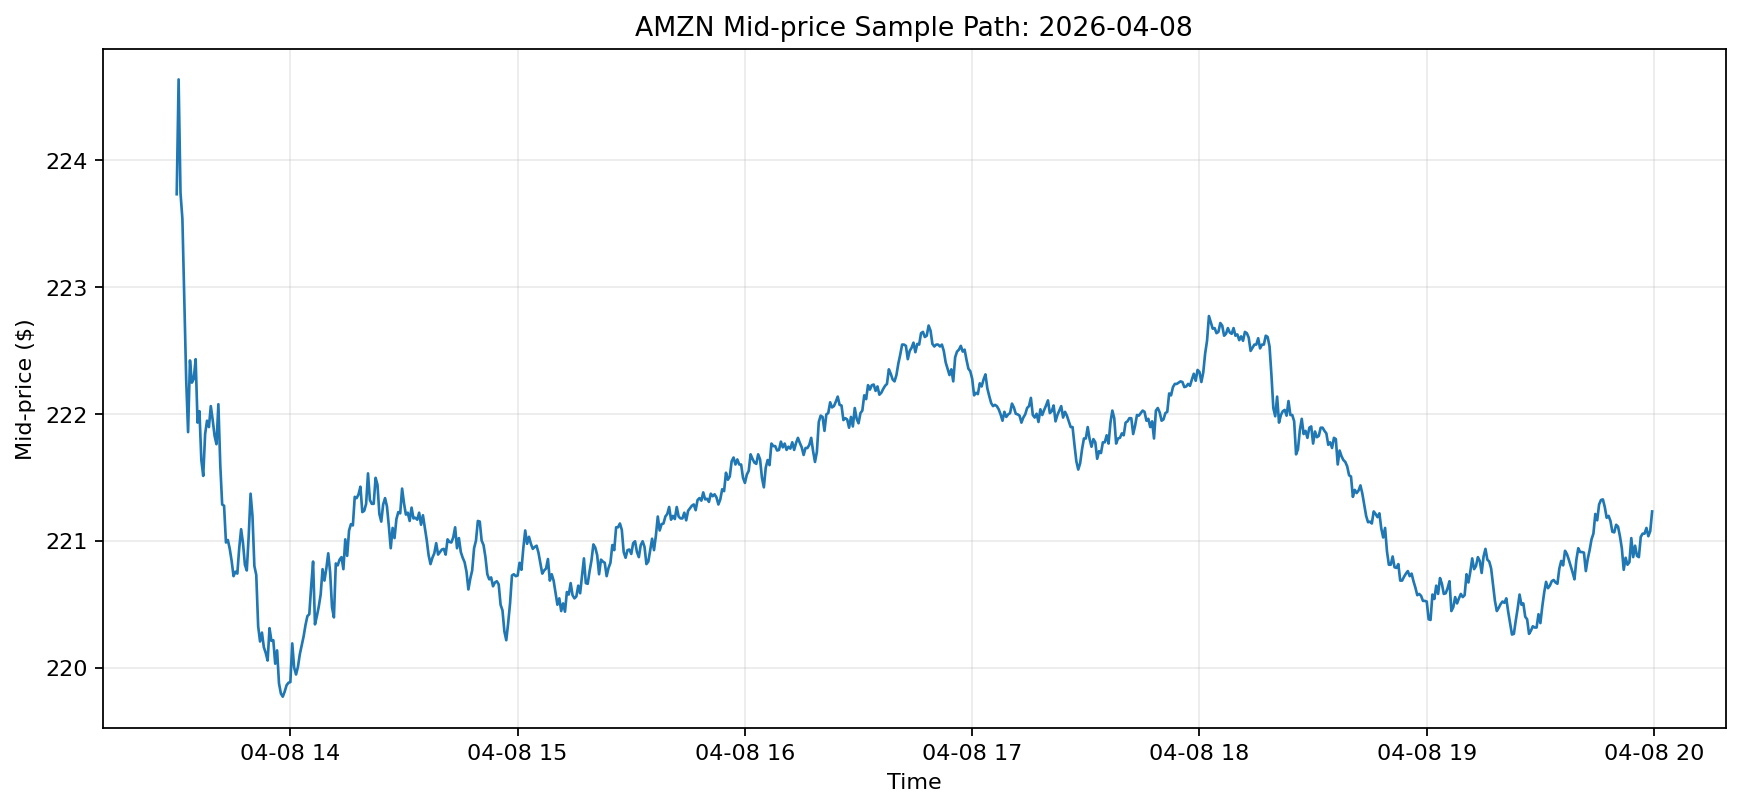
\includegraphics[width=0.75\textwidth]{figures/as/01_midprice_sample_path.png}
    \caption{AMZN mid-price sample path for the held-out test date 2026-04-08. This path is used as a representative diagnostic replay day, not as a full performance evaluation.}
    \label{fig:as-midprice-sample-path}
\end{figure}

Figure~\ref{fig:as-midprice-sample-path} shows the mid-price trajectory used for the representative diagnostic replay. The mid-price starts above \$224, falls rapidly toward approximately \$220, then partially recovers and fluctuates around \$221--\$223 for the remainder of the session. Since the AS model does not forecast the direction of the mid-price, this path is useful for a basic implementation check: the quotes should update with the mid-price and the inventory mechanism should remain interpretable under non-flat intraday movement.

\begin{figure}[htbp]
    \centering
    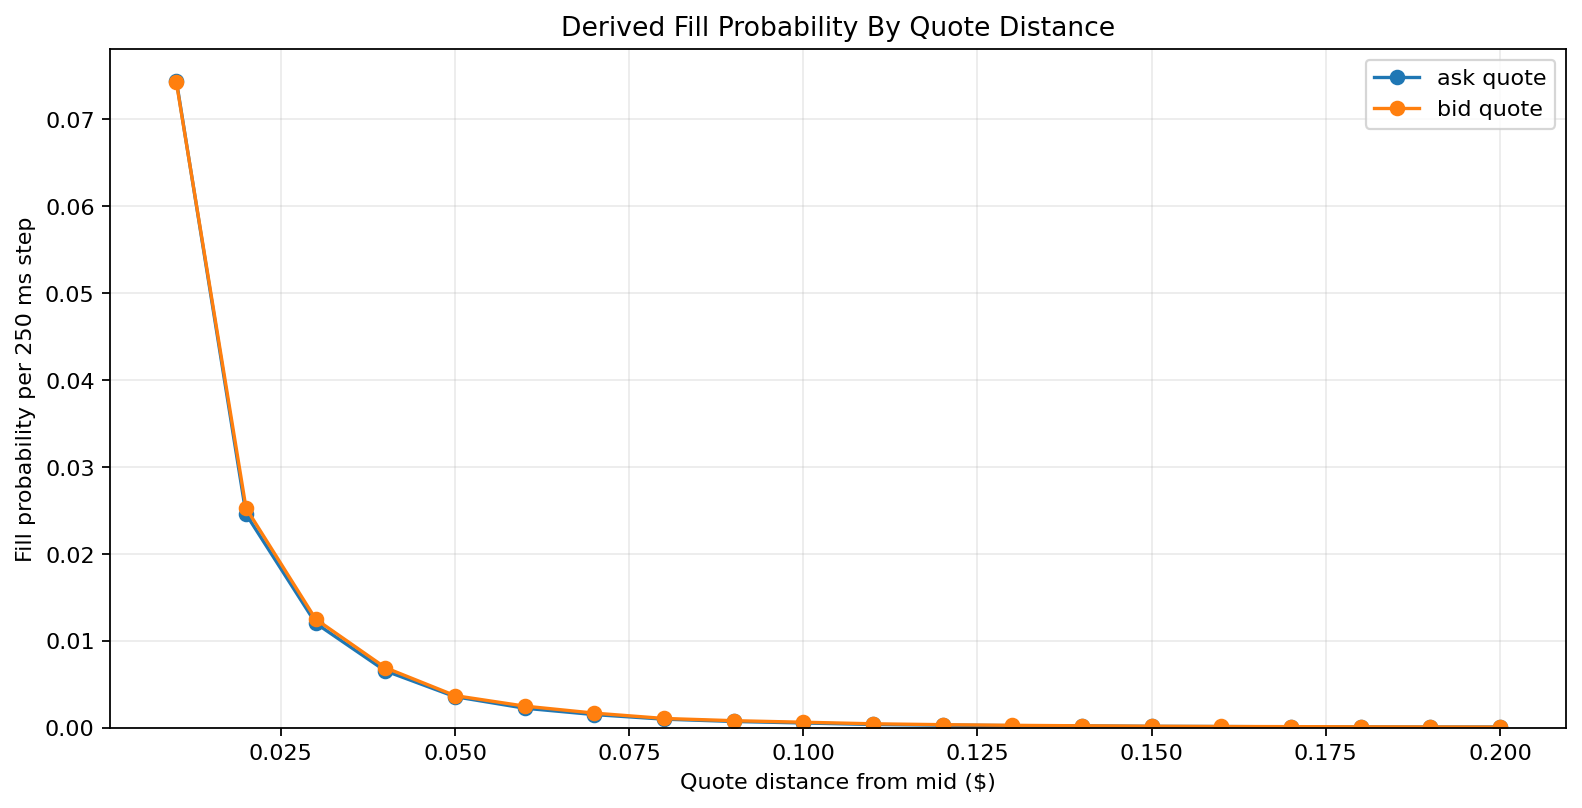
\includegraphics[width=0.75\textwidth]{figures/as/02_fill_probability_vs_distance.png}
    \caption{Derived fill probability per 250 ms decision step as a function of quote distance from the mid-price. The curve is used as a preliminary check for the distance-based arrival model.}
    \label{fig:as-fill-probability-distance}
\end{figure}

Figure~\ref{fig:as-fill-probability-distance} reports the empirical fill-probability curve used to motivate the exponential arrival-intensity model. Fill probability is highest close to the mid-price and decays quickly as the quote is moved away. The near overlap between the bid and ask curves suggests that a symmetric distance-based arrival model is a reasonable first approximation for this introductory benchmark. The curve should not be interpreted as a complete model of AMZN order flow.

\begin{figure}[htbp]
    \centering
    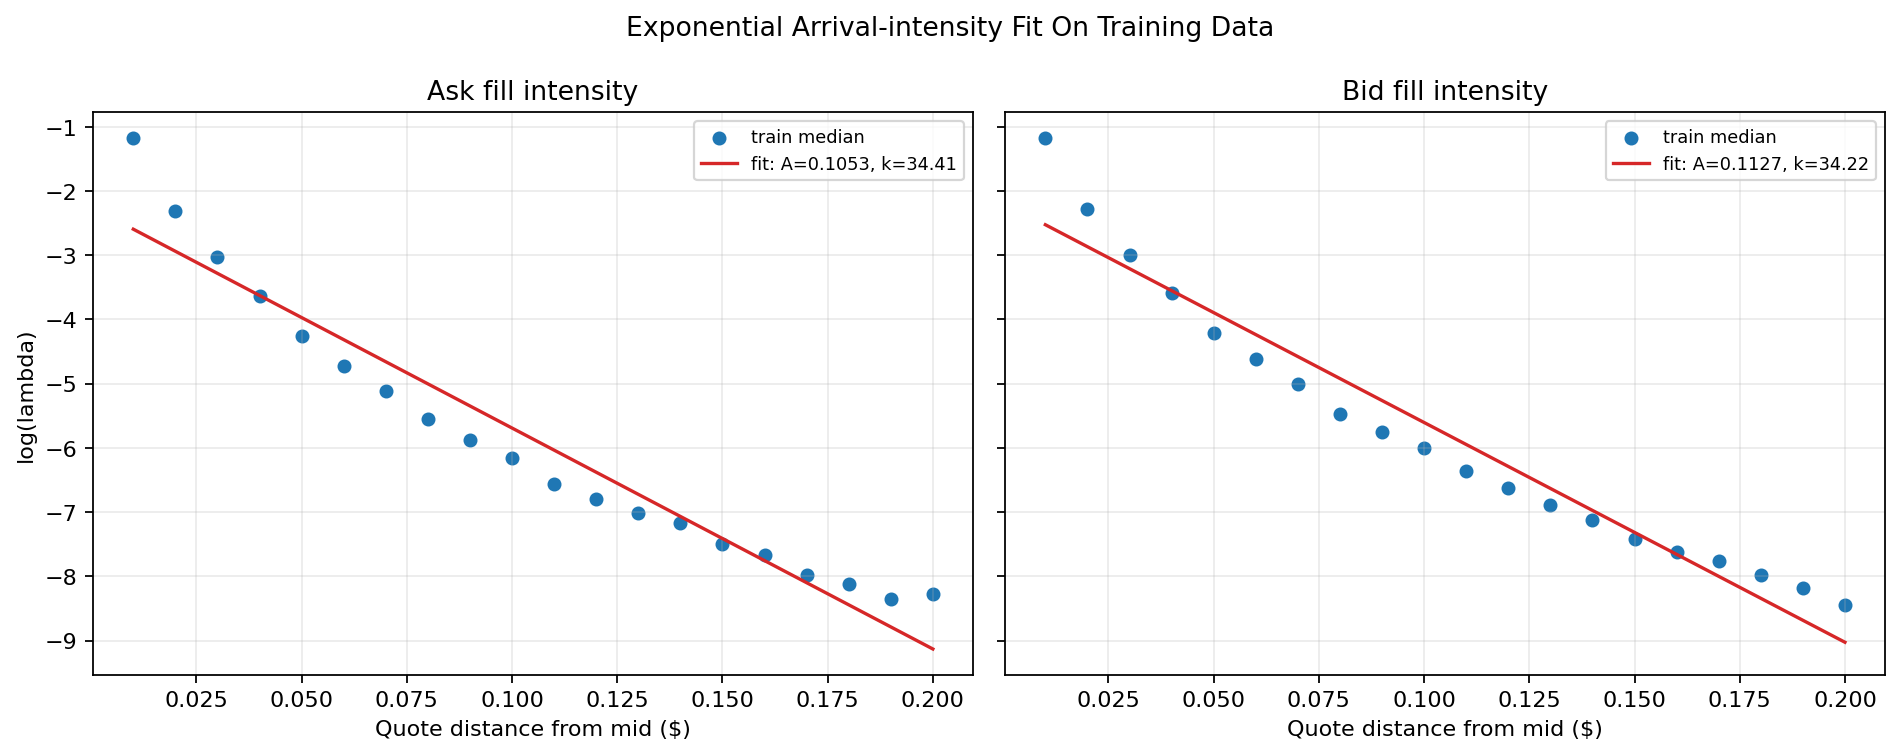
\includegraphics[width=0.75\textwidth]{figures/as/03_log_arrival_intensity_fit.png}
    \caption{Log arrival-intensity fit on the training data. The approximately linear pattern in log-space supports using $\lambda(\delta)=Ae^{-k\delta}$ as a simple preliminary benchmark assumption.}
    \label{fig:as-log-arrival-fit}
\end{figure}

The log-intensity plots in Figure~\ref{fig:as-log-arrival-fit} provide a direct visual check of the exponential assumption. In log-space, an exponential arrival model should be approximately linear in quote distance. The fitted ask and bid curves have similar slopes, with reported trade-through fits around $k\approx 34$ and arrival scales around $A\approx 0.105$--$0.113$. This supports using a simple calibrated distance-decay parameter for the preliminary AS benchmark, while the deviations at very short and very long quote distances show that the model remains approximate.

\begin{figure}[htbp]
    \centering
    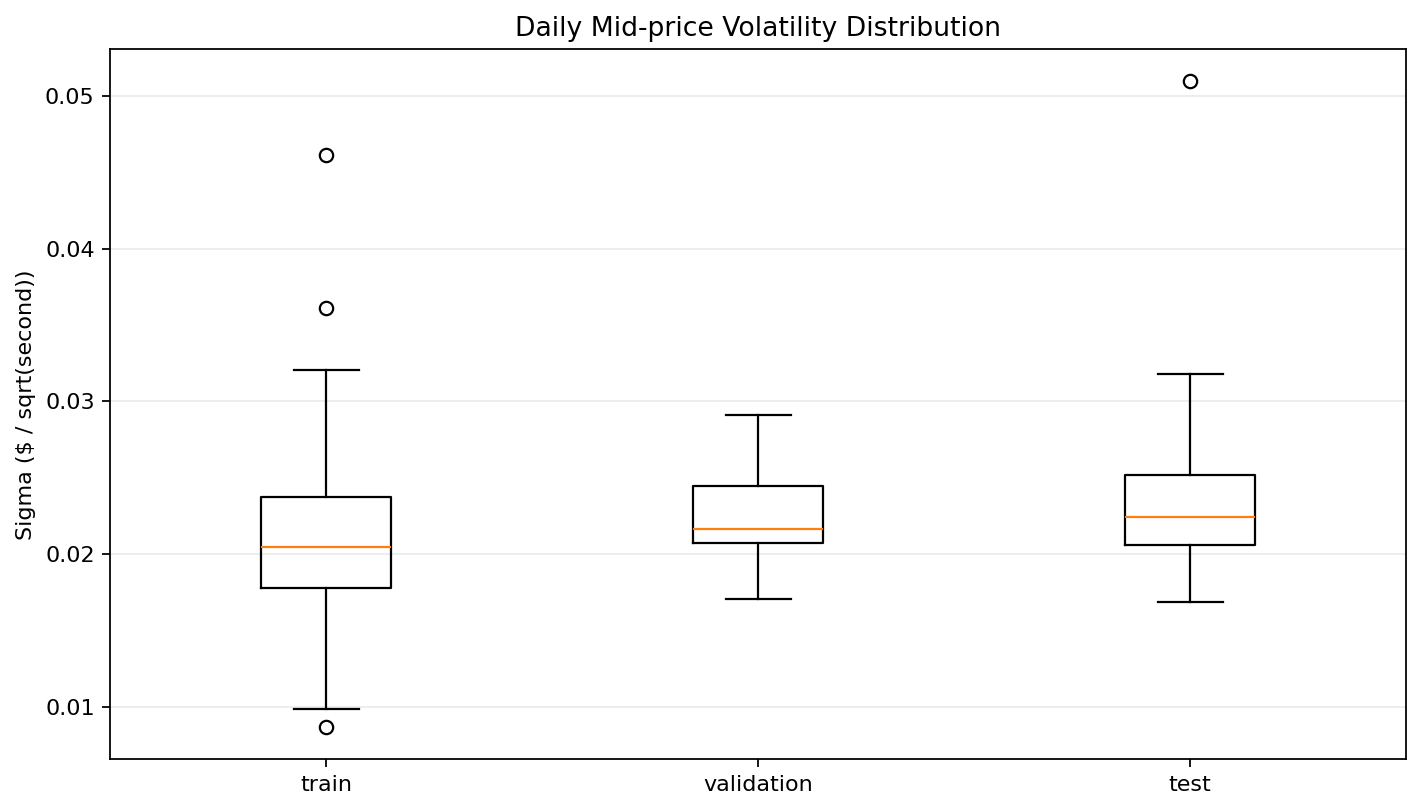
\includegraphics[width=0.8\textwidth]{figures/as/04_daily_volatility_distribution.png}
    \caption{Daily mid-price volatility distribution across train, validation, and test splits. This plot is used to check whether the held-out periods are broadly comparable to the training period.}
    \label{fig:as-daily-volatility-distribution}
\end{figure}

Figure~\ref{fig:as-daily-volatility-distribution} compares the volatility distributions across the chronological data splits. The test median is slightly above the training median, and the test set contains one large outlier. This is useful for later evaluation because the AS benchmark and the RL market maker should face the same out-of-sample variation. However, this diagnostic alone is not meant to establish final benchmark performance.

\subsection{Preliminary Experiment 2: Single-day inventory-aware replay}
\label{subsec:as-exp2}

Preliminary Experiment~2 runs the inventory-aware AS strategy on one held-out date, 2026-04-08. The goal is to inspect whether the replay code, inventory updates, quote construction, and marked-to-market accounting behave sensibly on a concrete example. The episode covers the full regular trading window from 13:30:00 to 19:59:59.750000 UTC at a 250 ms decision interval, resulting in 93,600 replay rows. Table~\ref{tab:as-exp2-summary} summarises the main diagnostic quantities for this representative day.

\begin{table}[htbp]
    \centering
    \caption{Preliminary single-day diagnostic summary for the inventory-aware AS replay on 2026-04-08.}
    \label{tab:as-exp2-summary}
    \small
    \begin{tabular}{lr}
        \toprule
        Quantity & Value \\
        \midrule
        Replay rows & 93,600 \\
        Final inventory & 40 shares \\
        Maximum absolute inventory & 100 shares \\
        Average squared inventory & 294.57 \\
        Root average squared inventory & 17.16 shares \\
        Final cash & -\$8,922.80 \\
        Final marked-to-market PnL & -\$72.00 \\
        Mean marked-to-market PnL & -\$101.97 \\
        \bottomrule
    \end{tabular}
\end{table}

The final marked-to-market PnL for this single diagnostic day is negative, at -\$72.00. This value is reported only to check the accounting scale and to illustrate that the replay produces non-trivial PnL paths. It should not be treated as evidence that the AS benchmark is profitable or unprofitable overall. A final performance claim would require evaluation over all held-out test days and a consistent comparison with the RL policy.

\begin{figure}[htbp]
    \centering
    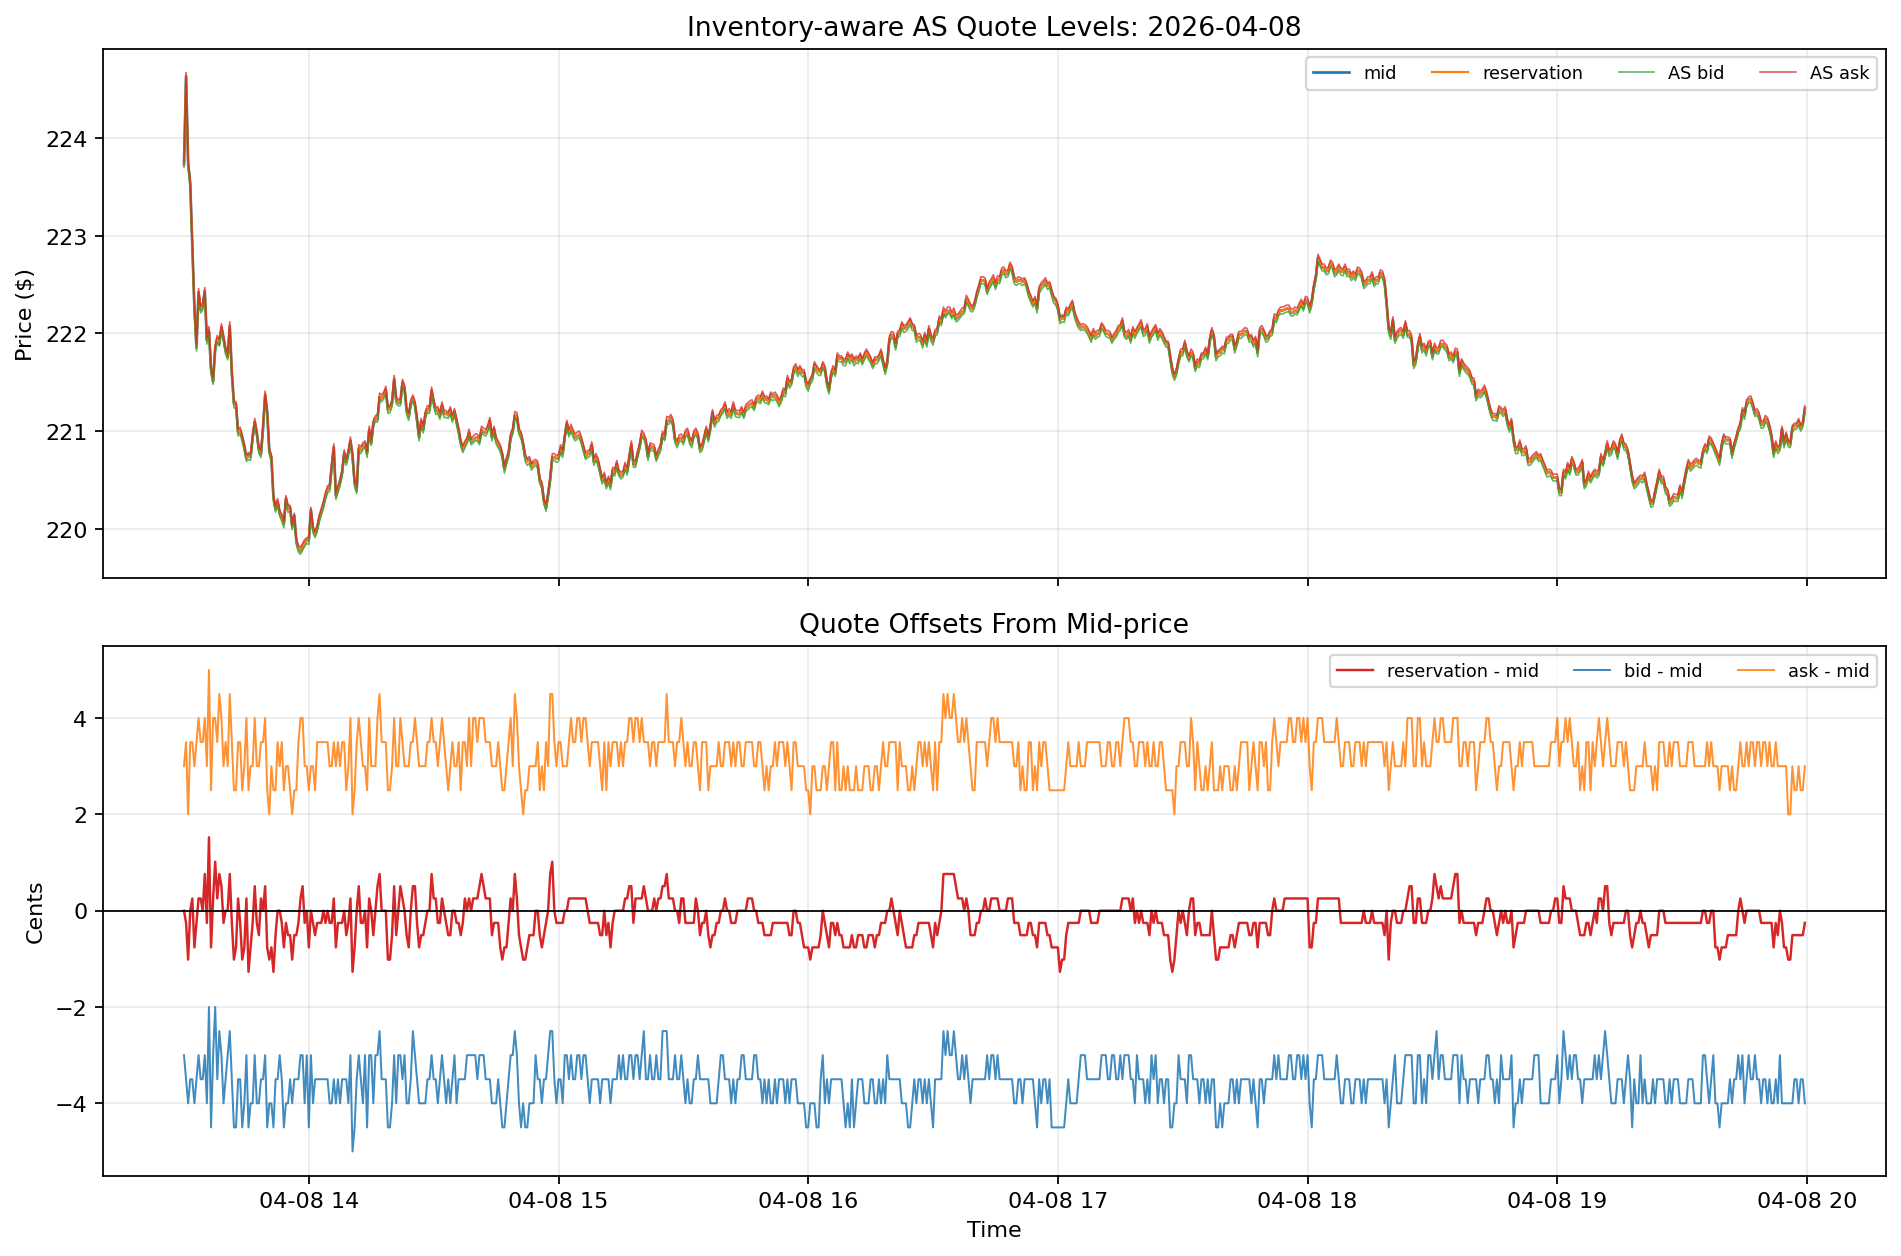
\includegraphics[width=0.98\textwidth]{figures/as/05_episode_quotes.png}
    \caption{Inventory-aware AS quote levels and quote offsets on 2026-04-08. The plot is used to inspect the implemented quote construction on a representative replay day.}
    \label{fig:as-episode-quotes}
\end{figure}

Figure~\ref{fig:as-episode-quotes} shows the central AS quoting mechanism in replay. The bid and ask quotes track the mid-price closely while remaining several cents away from it. The lower panel shows that the ask offset is typically around +3 to +4 cents and the bid offset around -3 to -4 cents, consistent with a calibrated spread of several ticks. The reservation-price offset is much smaller and oscillates around zero. This is consistent with the small AS risk-aversion setting: inventory moves the quote centre, but the shift is usually smaller than the base spread. Because this replay uses a rolling-horizon AS rule rather than the finite-horizon $T-t$ formulation, the plot should not be interpreted as evidence of terminal-time quote convergence.

\begin{figure}[htbp]
    \centering
    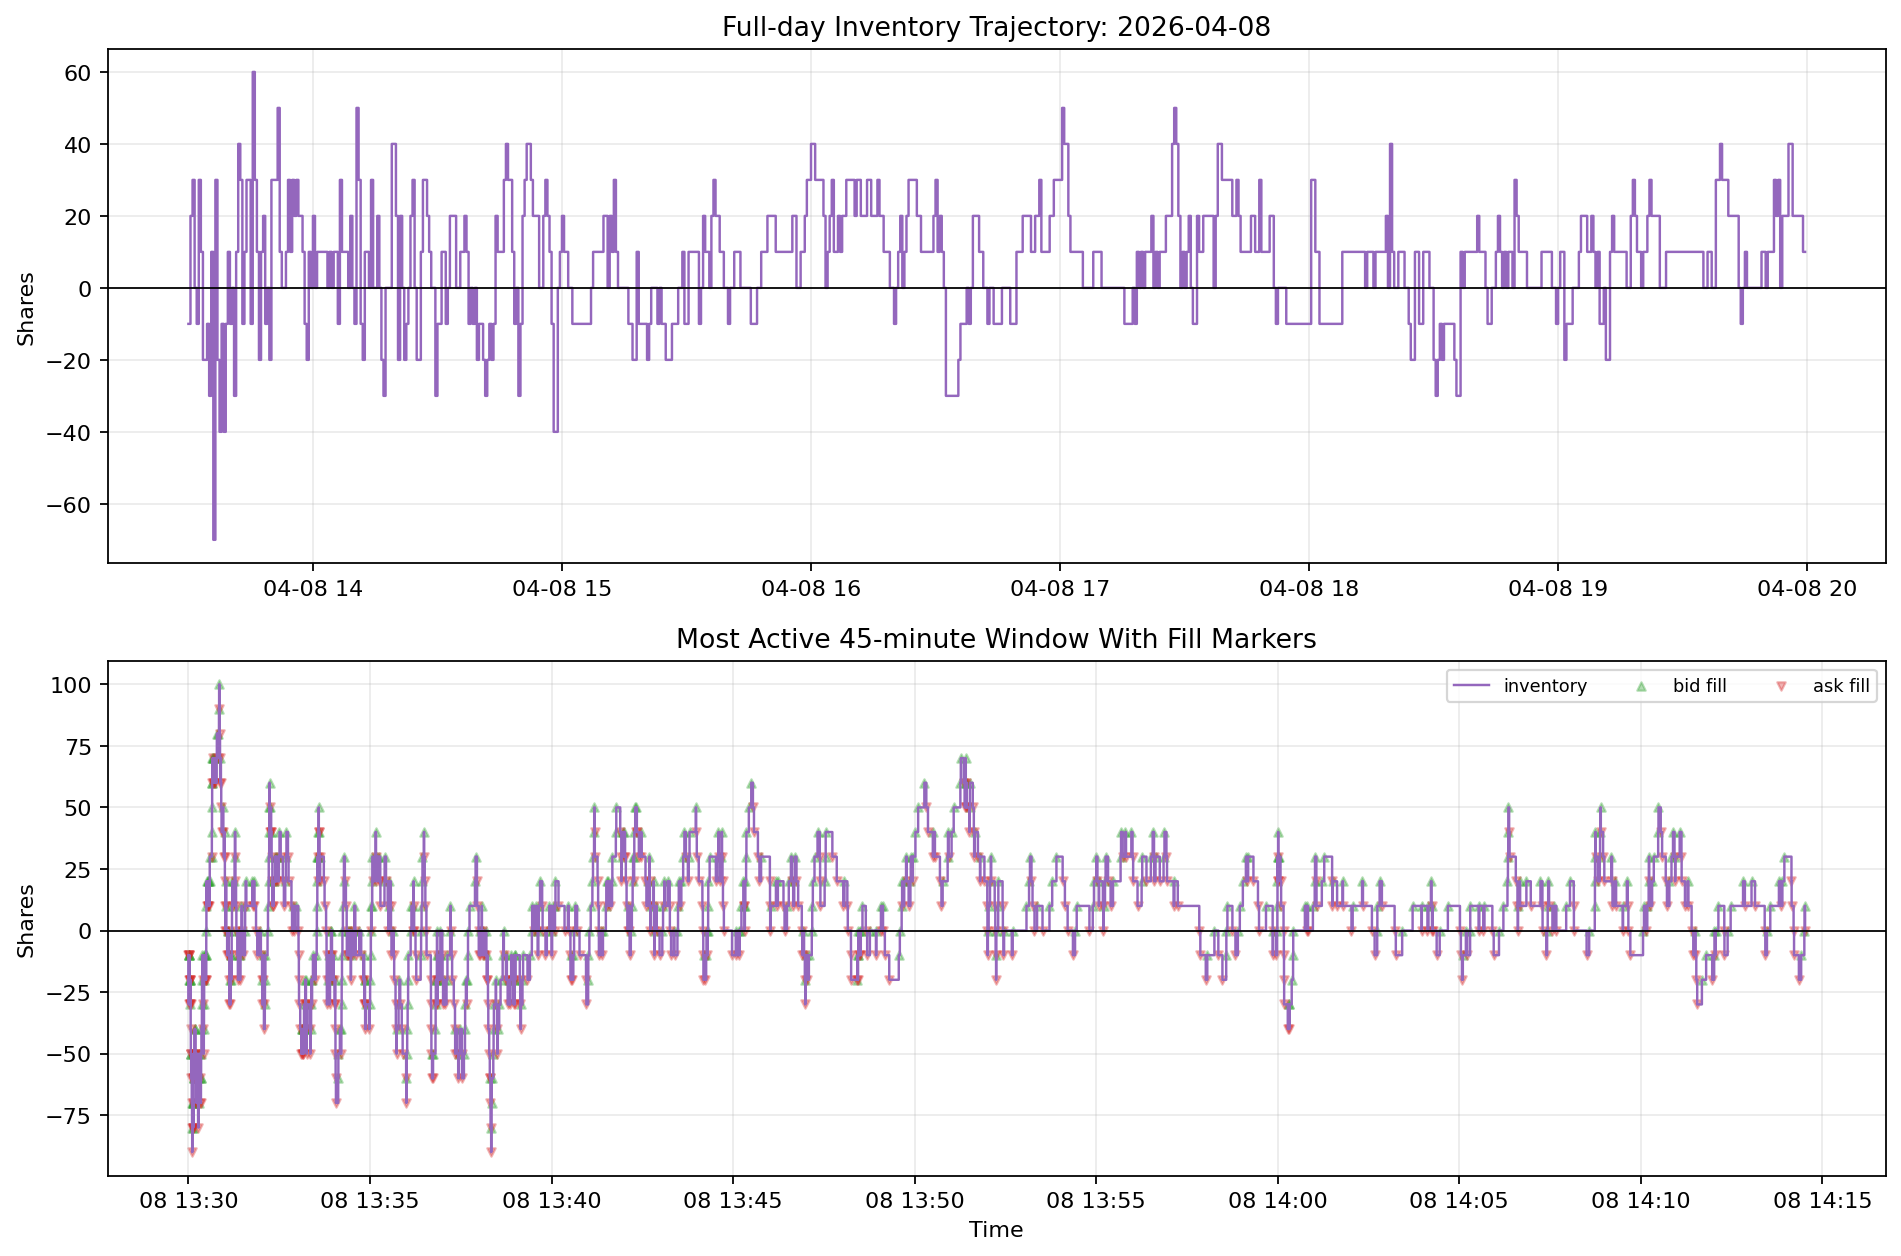
\includegraphics[width=0.98\textwidth]{figures/as/06_episode_inventory.png}
    \caption{Inventory trajectory and fill detail for the inventory-aware AS replay. The figure is used as a qualitative check that the policy trades and updates inventory in both directions.}
    \label{fig:as-episode-inventory}
\end{figure}

The inventory trajectory in Figure~\ref{fig:as-episode-inventory} shows that the AS strategy trades during the replay rather than simply remaining inactive. Inventory fluctuates around zero for much of the session, with a maximum absolute inventory of 100 shares and an average squared inventory of 294.57. The root average squared inventory is therefore approximately 17.16 shares, which gives a more interpretable scale for the typical inventory exposure. The zoomed panel shows alternating bid and ask fills in the most active window, which is a useful implementation check for two-sided passive trading.

\begin{figure}[htbp]
    \centering
    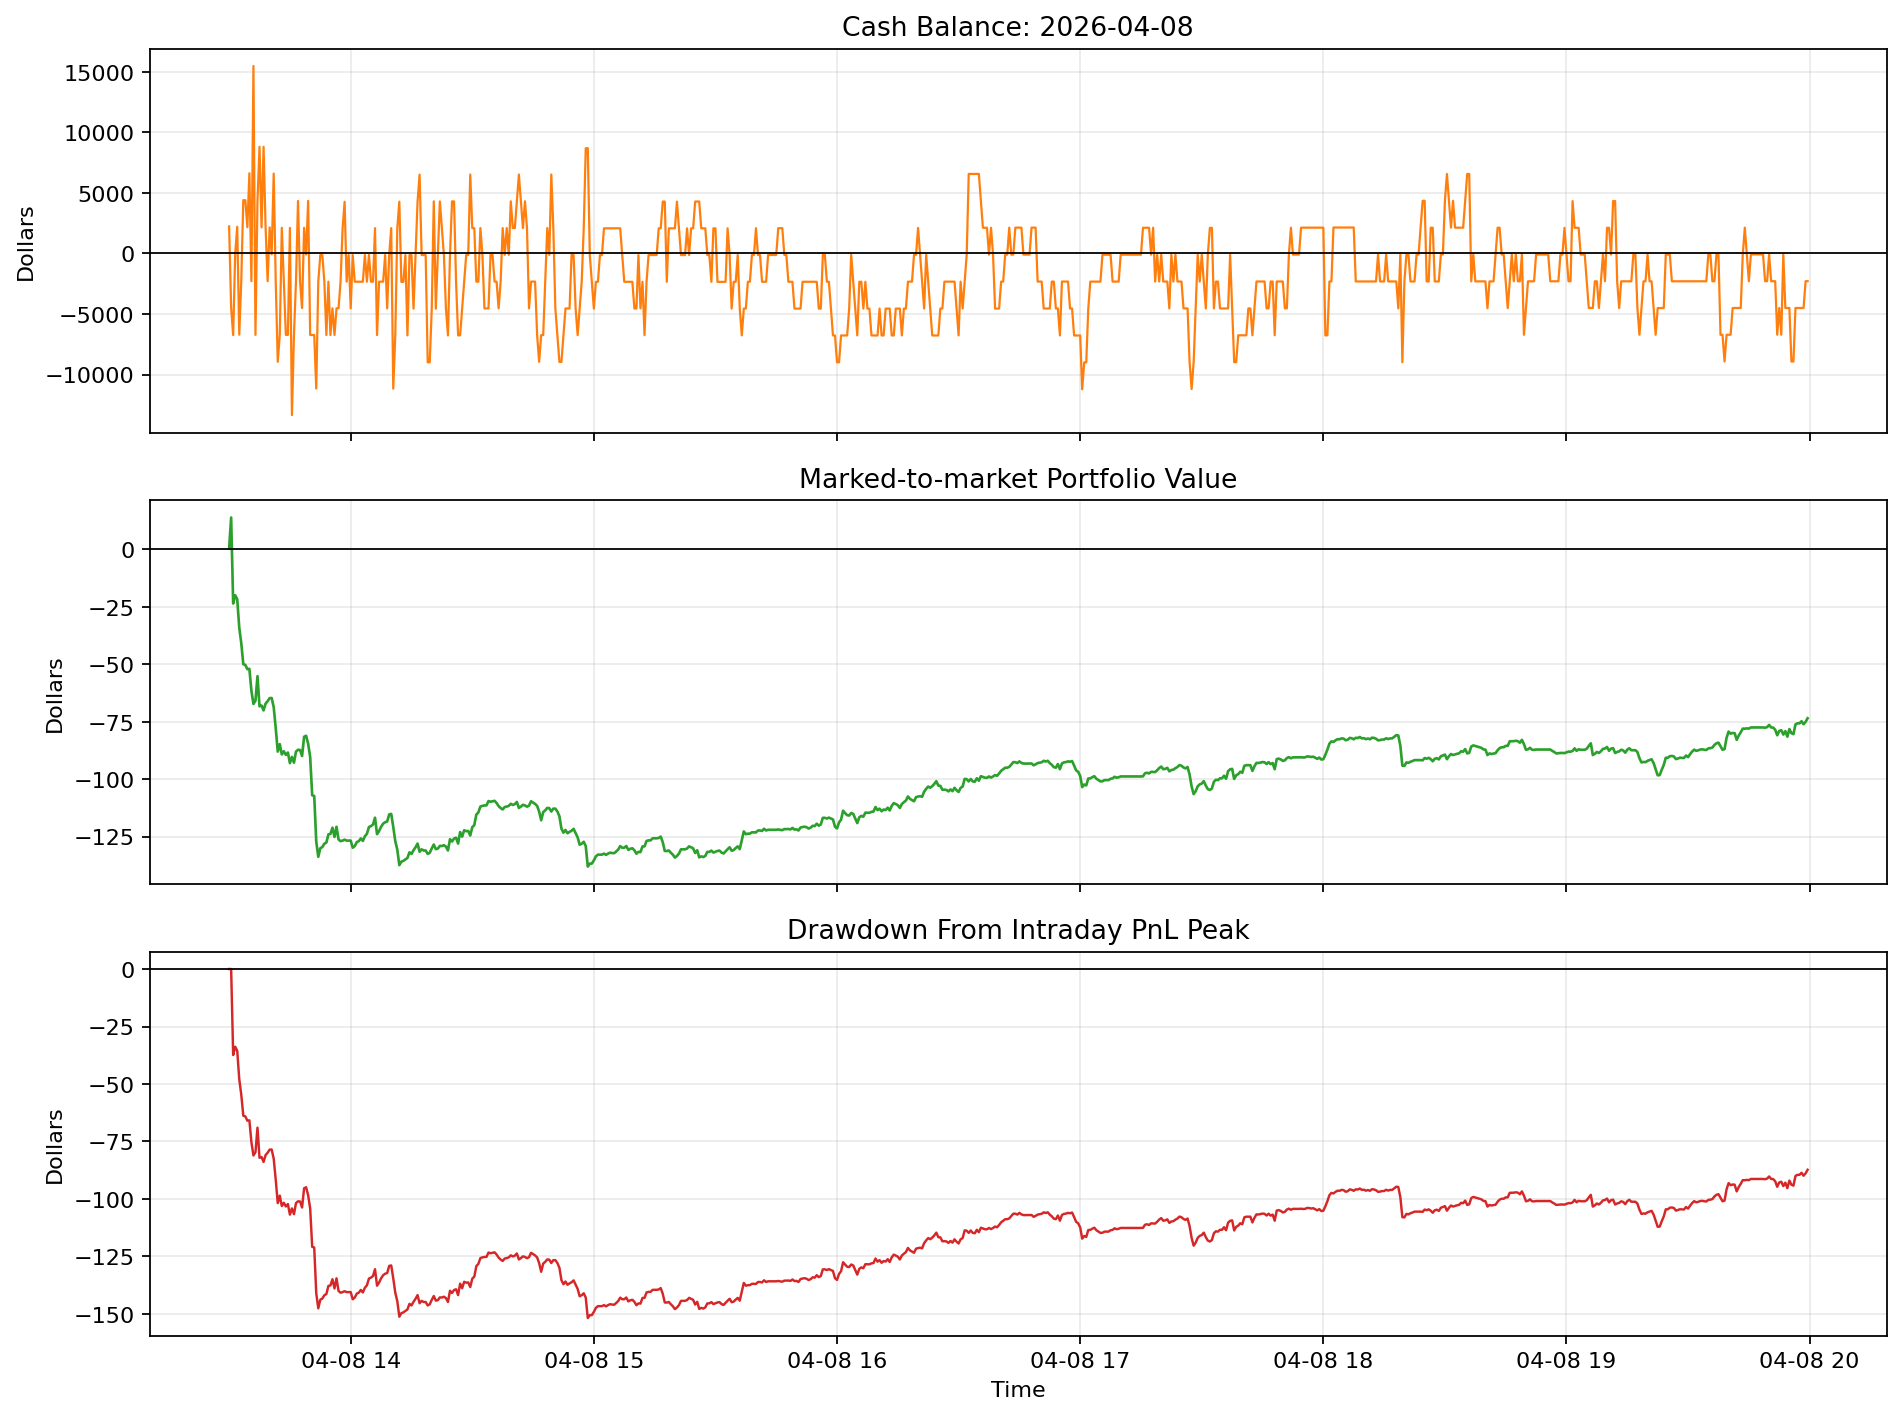
\includegraphics[width=0.98\textwidth]{figures/as/07_episode_cash_pnl.png}
    \caption{Cash balance, marked-to-market portfolio value, and drawdown from the intraday PnL peak for the AS replay on 2026-04-08. The figure illustrates the accounting convention used later for comparison.}
    \label{fig:as-episode-cash-pnl}
\end{figure}

Figure~\ref{fig:as-episode-cash-pnl} separates cash from marked-to-market portfolio value. Cash fluctuates strongly because every passive buy decreases cash and every passive sell increases cash. It should therefore not be interpreted as performance by itself. The relevant diagnostic metric is
\begin{equation}
    PV_t = C_t + Q_t m_t,
\end{equation}
where $C_t$ is cash, $Q_t$ is inventory, and $m_t$ is the mid-price. The portfolio-value curve falls sharply early in the day, reaches a drawdown of roughly -\$150, and then partially recovers to a final value of -\$72.00. For the present preliminary experiment, this mainly confirms that the replay produces a meaningful portfolio-value path and that drawdown should be included in the later RL comparison.

\begin{figure}[htbp]
    \centering
    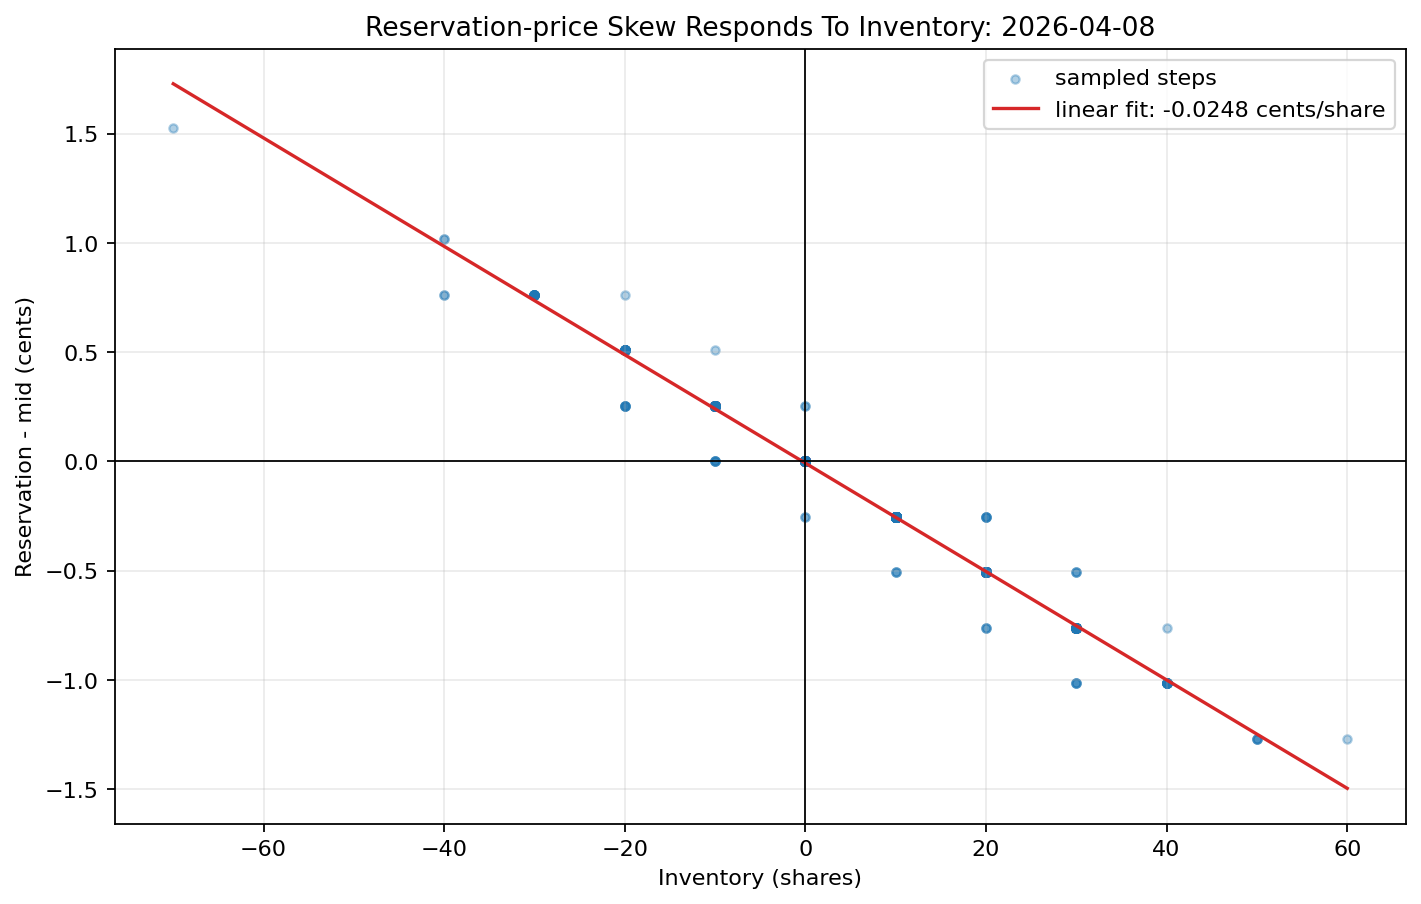
\includegraphics[width=0.85\textwidth]{figures/as/08_episode_skew_inventory_relationship.png}
    \caption{Relationship between inventory and reservation-price skew on 2026-04-08. The negative slope is a diagnostic check of the implemented AS inventory-skew mechanism.}
    \label{fig:as-skew-inventory-relationship}
\end{figure}

Figure~\ref{fig:as-skew-inventory-relationship} directly checks the AS inventory mechanism. The fitted relationship between inventory and reservation-price skew has slope -0.0248 cents per share. Thus, when the market maker is long, the reservation price is shifted below the mid-price, making selling relatively more attractive and buying relatively less attractive. When the market maker is short, the reservation price moves above the mid-price, encouraging inventory replenishment. This confirms the qualitative direction of the implemented AS skew on the representative replay day.

\subsection{Use of these diagnostics in the full experiment}
\label{subsec:as-rl-implications}

The two preliminary experiments above provide a starting point for the later reinforcement-learning evaluation. Experiment~1 checks that the fitted AS inputs have plausible magnitudes and that the train, validation, and test splits are broadly comparable. Experiment~2 checks that the AS replay produces interpretable quote skewing, inventory updates, cash movements, and marked-to-market portfolio values on one held-out day.

These checks are intentionally modest. They do not answer the main research question and they should not be presented as the final benchmark comparison. The full results section should later evaluate the learned RL market maker and execution agent across the planned risk-aversion sweeps, using metrics such as final portfolio value, portfolio-value variance, maximum absolute inventory, average squared inventory, fill rate, quoted spread, quote skew, drawdown, execution slippage, unfinished quantity, and cross-play outcomes. The AS diagnostics in this section simply provide a classical reference point and a sanity check for the accounting and replay pipeline used in those later comparisons.



\bibliographystyle{plain}
\bibliography{references}


\end{document}
